
\documentclass[UTF8,a4paper,12pt]{ctexart}

\usepackage{geometry}
\usepackage{amsmath,amssymb}
\usepackage{booktabs,longtable,array}
\usepackage{graphicx,float}
\graphicspath{{../../problems/D/q1/figures/}{problems/D/q1/figures/}}
\usepackage{xcolor}
\usepackage{tikz}
\usetikzlibrary{arrows.meta,positioning,calc,fit,patterns,shapes.geometric}
\usepackage{enumitem}
\usepackage{caption}
\usepackage{subcaption}
\usepackage[hidelinks]{hyperref}

\geometry{left=2.6cm,right=2.6cm,top=2.5cm,bottom=2.5cm}
\setlength{\parindent}{2em}
\setlength{\parskip}{0.25em}
\renewcommand{\arraystretch}{1.18}
\setcounter{tocdepth}{2}
\setcounter{secnumdepth}{3}

\newcommand{\figplaceholder}[2][5.2cm]{%
  \begin{figure}[H]
    \centering
    \fbox{\parbox[c][#1][c]{0.92\textwidth}{\centering #2}}
  \end{figure}
}

\title{山区洪涝救援中无人机运输--通信协同调度与独立资源配置}
\author{}
\date{}

% Q2-EVIDENCE-V7-FOCUSED formal manuscript figures.
% Auto-generated from paper/data/q2_v7_visual_source.json.
% No legacy q2_closing figure is used by these macros.
\definecolor{qLight}{HTML}{E4E8EB}
\definecolor{qLMid}{HTML}{C4CDD3}
\definecolor{qMid}{HTML}{98A8B2}
\definecolor{qDark}{HTML}{657A87}
\definecolor{qDeep}{HTML}{3F5663}
\definecolor{qText}{HTML}{30343A}
\definecolor{qGrid}{HTML}{D9DDE0}

\newcommand{\QTwoFigFramework}{%
\begin{tikzpicture}[>=Latex,font=\small]
\node[draw=qDark,fill=qLight,rounded corners=2pt,minimum width=5.0cm,minimum height=.8cm,align=center] (a) at (0,4.9) {Q1安全可行批型 / 候选运输任务};
\node[draw=qDark,fill=qLight,rounded corners=2pt,minimum width=6.2cm,minimum height=1.05cm,align=center] (b) at (0,3.5) {多点运输任务构造\\箱组 · 访问顺序 · 机型 · 时长 · 能耗 · 箱级送达偏移};
\node[draw=qDark,fill=qLMid,rounded corners=2pt,minimum width=6.2cm,minimum height=1.05cm,align=center] (c) at (0,2.0) {飞机--电池联合资源排程\\实体飞机 · 共享电池 · 充电恢复 · deadline · 开始时刻};
\node[draw=qDark,fill=qLight,rounded corners=2pt,minimum width=5.2cm,minimum height=1.35cm,align=center] (u) at (-3.7,.25) {可行上界路线\\任务重构 $\to$ 事件排程 $\to$ 独立重放\\得到真实可执行 UB};
\node[draw=qDark,fill=qLight,rounded corners=2pt,minimum width=5.2cm,minimum height=1.35cm,align=center] (l) at (3.7,.25) {全局下界路线\\任务列松弛 $\to$ 完整定价 $\to$ 分支覆盖证书\\得到有效 LB};
\node[draw=qDark,fill=qLMid,rounded corners=2pt,minimum width=5.4cm,minimum height=.85cm,align=center] (z) at (0,-1.45) {确定性认证区间：$LB\le T^*\le UB$};
\draw[->,qDark] (a)--(b); \draw[->,qDark] (b)--(c); \draw[->,qDark] (c)--(u); \draw[->,qDark] (c)--(l); \draw[->,qDark] (u)--(z); \draw[->,qDark] (l)--(z);
\node[qDark,font=\footnotesize,align=center] at (0,-2.25) {同时回答“方案能否真实执行”与“当前方案距离理论下界还有多远”};
\end{tikzpicture}}

\newcommand{\QTwoFigOccupancy}{%
\begin{tikzpicture}[x=1.05cm,y=1cm,font=\small]
\foreach \x/\lab in {1/任务开始,7/返航,9/电池恢复满电}{\draw[dashed,qGrid] (\x,.25)--(\x,2.15); \node[font=\footnotesize] at (\x,2.38){\lab};}
\node[anchor=east] at (.65,1.65){运输无人机}; \node[anchor=east] at (.65,.75){共享电池};
\fill[qDark] (1,1.4) rectangle (7,1.9); \node[white] at (4,1.65){准备 + 飞行 + 配送 + 返航};
\fill[qDark] (1,.5) rectangle (7,1.0); \node[white] at (4,.75){任务占用};
\fill[qLMid] (7,.5) rectangle (9,1.0); \node[qText] at (8,.75){充电恢复};
\node[qDark,font=\footnotesize] at (4,1.22){$I_r^U=[s_r,s_r+p_r)$};
\node[qDark,font=\footnotesize] at (5,.32){$I_r^B=[s_r,s_r+p_r+c_r)$};
\node[qDark,font=\footnotesize] at (5,-.05){飞机返航后释放，而原电池继续占用至恢复满电};
\end{tikzpicture}}

\newcommand{\QTwoFigUpperSearch}{%
\begin{tikzpicture}[>=Latex,font=\small,node distance=8mm]
\tikzset{bx/.style={draw=qDark,fill=qLight,rounded corners=2pt,minimum width=7.4cm,minimum height=.9cm,align=center}, strong/.style={bx,fill=qLMid}}
\node[strong] (a) {当前完整可行方案};
\node[bx,below=of a] (b) {识别关键链：迟到风险 · makespan瓶颈 · 飞机链 · 电池链};
\node[bx,below=of b] (c) {构造重构邻域：货箱重分配 · 路线重构 · 机型调整 · 资源链释放};
\node[bx,below=of c] (d) {快速物理筛选：质量 · 体积 · 能量 · 时限必要条件};
\node[strong,below=of d] (e) {精确事件排程 + 独立重放：飞机 · 电池 · 充电 · 箱级deadline};
\node[bx,below=of e,minimum width=3.2cm] (g) {严格改善？};
\draw[->,qDark] (a)--(b);\draw[->,qDark](b)--(c);\draw[->,qDark](c)--(d);\draw[->,qDark](d)--(e);\draw[->,qDark](e)--(g);
\node[right=18mm of g,qDark] (yes) {是：接受为新UB}; \draw[->,qDark] (g)--(yes);
\node[left=18mm of g,qDark] (no) {否：拒绝并换邻域}; \draw[->,qDark] (g)--(no);
\draw[->,qDark] (no.west) -- ++(-.7,0) |- (c.west);
\node[qDark,font=\footnotesize,below=5mm of g,align=center] {候选必须经过完整事件排程与重放后才能成为正式可行上界};
\end{tikzpicture}}

\newcommand{\QTwoFigRouteMap}{%
\begin{tikzpicture}[x=.85cm,y=.85cm,font=\footnotesize]
\draw[->,qText] (-6.9,-.8)--(6.2,-.8) node[right]{AEQD $x$/km};
\draw[->,qText] (-6.9,-.8)--(-6.9,8.35) node[above]{AEQD $y$/km};
\draw[qLMid,line width=.65pt,opacity=.78] (0.000,0.000) -- (1.269,2.778) -- (0.000,0.000);
\draw[qLMid,line width=.65pt,opacity=.78] (0.000,0.000) -- (0.750,7.678) -- (0.000,0.000);
\draw[qLMid,line width=.65pt,opacity=.78] (0.000,0.000) -- (4.155,2.501) -- (0.000,0.000);
\draw[qLMid,line width=.65pt,opacity=.78] (0.000,0.000) -- (-1.078,2.593) -- (0.750,7.678) -- (0.000,0.000);
\draw[qDark,dashed,line width=.65pt,opacity=.78] (0.000,0.000) -- (4.630,1.207) -- (0.000,0.000);
\draw[qDark,dashed,line width=.65pt,opacity=.78] (0.000,0.000) -- (5.407,-0.364) -- (0.000,0.000);
\draw[qMid,dotted,line width=.65pt,opacity=.78] (0.000,0.000) -- (1.269,2.778) -- (0.000,0.000);
\draw[qMid,dotted,line width=.65pt,opacity=.78] (0.000,0.000) -- (1.269,2.778) -- (0.000,0.000);
\draw[qLMid,line width=.65pt,opacity=.78] (0.000,0.000) -- (2.387,5.182) -- (2.838,6.846) -- (4.155,2.501) -- (0.000,0.000);
\draw[qMid,dotted,line width=.65pt,opacity=.78] (0.000,0.000) -- (-3.185,-0.088) -- (0.000,0.000);
\draw[qDark,dashed,line width=.65pt,opacity=.78] (0.000,0.000) -- (5.358,5.090) -- (0.000,0.000);
\draw[qLMid,line width=.65pt,opacity=.78] (0.000,0.000) -- (-3.898,2.316) -- (0.000,0.000);
\draw[qMid,dotted,line width=.65pt,opacity=.78] (0.000,0.000) -- (2.838,6.846) -- (0.000,0.000);
\draw[qDark,dashed,line width=.65pt,opacity=.78] (0.000,0.000) -- (0.750,7.678) -- (0.000,0.000);
\draw[qLMid,line width=.65pt,opacity=.78] (0.000,0.000) -- (-3.898,2.316) -- (0.000,0.000);
\draw[qLMid,line width=.65pt,opacity=.78] (0.000,0.000) -- (-6.354,3.519) -- (-3.943,4.535) -- (0.000,0.000);
\draw[qMid,dotted,line width=.65pt,opacity=.78] (0.000,0.000) -- (-3.898,2.316) -- (-6.354,3.519) -- (0.000,0.000);
\draw[qDark,dashed,line width=.65pt,opacity=.78] (0.000,0.000) -- (-1.855,7.863) -- (0.000,0.000);
\draw[qLMid,line width=.65pt,opacity=.78] (0.000,0.000) -- (-3.943,4.535) -- (0.000,0.000);
\draw[qDark,dashed,line width=.65pt,opacity=.78] (0.000,0.000) -- (-1.855,7.863) -- (0.000,0.000);
\draw[qMid,dotted,line width=.65pt,opacity=.78] (0.000,0.000) -- (-0.261,5.274) -- (0.000,0.000);
\draw[qLMid,line width=.65pt,opacity=.78] (0.000,0.000) -- (2.387,5.182) -- (0.000,0.000);
\draw[qLMid,line width=.65pt,opacity=.78] (0.000,0.000) -- (-1.078,2.593) -- (0.000,0.000);
\node[star,star points=5,fill=qDeep,minimum size=5pt,inner sep=1.2pt,label={below right:O01}] at (0,0) {};
\fill[qDeep] (1.269,2.778) circle (1.25pt); \node[anchor=south west] at (1.369,2.838) {S001};
\fill[qDeep] (2.838,6.846) circle (1.25pt); \node[anchor=south west] at (2.938,6.906) {S002};
\fill[qDeep] (-6.354,3.519) circle (1.25pt); \node[anchor=south west] at (-6.254,3.579) {S003};
\fill[qDeep] (0.750,7.678) circle (1.25pt); \node[anchor=south west] at (0.850,7.738) {S004};
\fill[qDeep] (-0.261,5.274) circle (1.25pt); \node[anchor=south west] at (-0.161,5.334) {S005};
\fill[qDeep] (-3.185,-0.088) circle (1.25pt); \node[anchor=south west] at (-3.085,-0.028) {S006};
\fill[qDeep] (-3.898,2.316) circle (1.25pt); \node[anchor=south west] at (-3.798,2.376) {S007};
\fill[qDeep] (-1.855,7.863) circle (1.25pt); \node[anchor=south west] at (-1.755,7.923) {S008};
\fill[qDeep] (2.387,5.182) circle (1.25pt); \node[anchor=south west] at (2.487,5.242) {S009};
\fill[qDeep] (4.630,1.207) circle (1.25pt); \node[anchor=south west] at (4.730,1.267) {S010};
\fill[qDeep] (-1.078,2.593) circle (1.25pt); \node[anchor=south west] at (-0.978,2.653) {S011};
\fill[qDeep] (5.358,5.090) circle (1.25pt); \node[anchor=south west] at (5.458,5.150) {S012};
\fill[qDeep] (4.155,2.501) circle (1.25pt); \node[anchor=south west] at (4.255,2.561) {S013};
\fill[qDeep] (5.407,-0.364) circle (1.25pt); \node[anchor=south west] at (5.507,-0.304) {S014};
\fill[qDeep] (-3.943,4.535) circle (1.25pt); \node[anchor=south west] at (-3.843,4.595) {S015};
\node[qDark,anchor=north west,font=\small] at (-6.65,8.1){23架次；A/B/C=11/6/6};
\draw[qLMid,line width=.8pt] (1.45,-.45)--(2.15,-.45) node[right,qText]{A型};
\draw[qDark,dashed,line width=.8pt] (3.0,-.45)--(3.7,-.45) node[right,qText]{B型};
\draw[qMid,dotted,line width=.8pt] (4.55,-.45)--(5.25,-.45) node[right,qText]{C型};
\end{tikzpicture}}

\newcommand{\QTwoFigGantt}{%
\begin{minipage}{.99\linewidth}\centering
\begin{tikzpicture}[x=.095cm,y=.48cm,font=\scriptsize]
\draw[qGrid] (0,0)--(0,8.6); \node[below] at (0,0) {0};
\draw[qGrid] (20,0)--(20,8.6); \node[below] at (20,0) {20};
\draw[qGrid] (40,0)--(40,8.6); \node[below] at (40,0) {40};
\draw[qGrid] (60,0)--(60,8.6); \node[below] at (60,0) {60};
\draw[qGrid] (80,0)--(80,8.6); \node[below] at (80,0) {80};
\draw[qGrid] (100,0)--(100,8.6); \node[below] at (100,0) {100};
\draw[qGrid] (120,0)--(120,8.6); \node[below] at (120,0) {120};
\draw[qGrid] (140,0)--(140,8.6); \node[below] at (140,0) {140};
\node[anchor=east] at (-1,8) {U01};
\node[anchor=east] at (-1,7) {U02};
\node[anchor=east] at (-1,6) {U03};
\node[anchor=east] at (-1,5) {U04};
\node[anchor=east] at (-1,4) {U05};
\node[anchor=east] at (-1,3) {U06};
\node[anchor=east] at (-1,2) {U07};
\node[anchor=east] at (-1,1) {U08};
\fill[qLMid] (0.000,7.68) rectangle (20.848,8.32); \node at (10.424,8) {R01};
\fill[qLMid] (0.000,6.68) rectangle (36.313,7.32); \node at (18.157,7) {R02};
\fill[qLMid] (0.000,5.68) rectangle (26.869,6.32); \node at (13.434,6) {R03};
\fill[qLMid] (0.000,4.68) rectangle (41.068,5.32); \node at (20.534,5) {R04};
\fill[qDark] (0.000,3.68) rectangle (25.923,4.32); \node at (12.961,4) {R05};
\fill[qDark] (0.000,2.68) rectangle (31.163,3.32); \node at (15.581,3) {R06};
\fill[qMid] (0.000,1.68) rectangle (27.103,2.32); \node at (13.551,2) {R07};
\fill[qMid] (0.000,0.68) rectangle (23.803,1.32); \node at (11.901,1) {R08};
\fill[qLMid] (20.848,7.68) rectangle (65.440,8.32); \node at (43.144,8) {R09};
\fill[qMid] (23.803,0.68) rectangle (49.829,1.32); \node at (36.816,1) {R10};
\fill[qDark] (25.923,3.68) rectangle (57.969,4.32); \node at (41.946,4) {R11};
\fill[qLMid] (26.869,5.68) rectangle (55.659,6.32); \node at (41.264,6) {R12};
\fill[qMid] (27.103,1.68) rectangle (63.333,2.32); \node at (45.218,2) {R13};
\fill[qDark] (31.163,2.68) rectangle (63.190,3.32); \node at (47.176,3) {R14};
\fill[qLMid] (36.313,6.68) rectangle (65.104,7.32); \node at (50.709,7) {R15};
\fill[qLMid] (44.954,4.68) rectangle (88.343,5.32); \node at (66.648,5) {R16};
\fill[qMid] (49.829,0.68) rectangle (94.722,1.32); \node at (72.275,1) {R17};
\fill[qDark] (57.969,3.68) rectangle (90.666,4.32); \node at (74.317,4) {R18};
\fill[qLMid] (60.011,5.68) rectangle (92.821,6.32); \node at (76.416,6) {R19};
\fill[qDark] (63.190,2.68) rectangle (94.887,3.32); \node at (79.039,3) {R20};
\fill[qMid] (63.333,1.68) rectangle (94.620,2.32); \node at (78.976,2) {R21};
\fill[qLMid] (65.104,6.68) rectangle (93.247,7.32); \node at (79.176,7) {R22};
\fill[qLMid] (73.166,7.68) rectangle (93.533,8.32); \node at (83.350,8) {R23};
\draw[qDeep,dashed,line width=.8pt] (94.887,.35)--(94.887,8.45);
\node[anchor=west,qDark] at (95.887,8.2){(a) 飞机占用};
\node[rotate=90] at (-4,4.5){运输无人机}; \node at (70,-.8){从调度开始计时 / min};
\end{tikzpicture}\par\smallskip
\begin{tikzpicture}[x=.095cm,y=.38cm,font=\scriptsize]
\draw[qGrid] (0,0)--(0,14.8); \node[below] at (0,0) {0};
\draw[qGrid] (20,0)--(20,14.8); \node[below] at (20,0) {20};
\draw[qGrid] (40,0)--(40,14.8); \node[below] at (40,0) {40};
\draw[qGrid] (60,0)--(60,14.8); \node[below] at (60,0) {60};
\draw[qGrid] (80,0)--(80,14.8); \node[below] at (80,0) {80};
\draw[qGrid] (100,0)--(100,14.8); \node[below] at (100,0) {100};
\draw[qGrid] (120,0)--(120,14.8); \node[below] at (120,0) {120};
\draw[qGrid] (140,0)--(140,14.8); \node[below] at (140,0) {140};
\node[anchor=east] at (-1,14) {A-BAT01};
\node[anchor=east] at (-1,13) {A-BAT02};
\node[anchor=east] at (-1,12) {A-BAT03};
\node[anchor=east] at (-1,11) {A-BAT04};
\node[anchor=east] at (-1,10) {A-BAT05};
\node[anchor=east] at (-1,9) {A-BAT06};
\node[anchor=east] at (-1,8) {B-BAT01};
\node[anchor=east] at (-1,7) {B-BAT02};
\node[anchor=east] at (-1,6) {B-BAT03};
\node[anchor=east] at (-1,5) {B-BAT04};
\node[anchor=east] at (-1,4) {C-BAT01};
\node[anchor=east] at (-1,3) {C-BAT02};
\node[anchor=east] at (-1,2) {C-BAT03};
\node[anchor=east] at (-1,1) {C-BAT04};
\fill[qLMid] (0.000,13.73) rectangle (20.848,14.27); \fill[qLight] (20.848,13.73) rectangle (35.356,14.27);
\fill[qLMid] (0.000,12.73) rectangle (36.313,13.27); \fill[qLight] (36.313,12.73) rectangle (60.011,13.27);
\fill[qLMid] (0.000,11.73) rectangle (26.869,12.27); \fill[qLight] (26.869,11.73) rectangle (44.954,12.27);
\fill[qLMid] (0.000,10.73) rectangle (41.068,11.27); \fill[qLight] (41.068,10.73) rectangle (64.930,11.27);
\fill[qDark] (0.000,7.73) rectangle (25.923,8.27); \fill[qLight] (25.923,7.73) rectangle (50.202,8.27);
\fill[qDark] (0.000,6.73) rectangle (31.163,7.27); \fill[qLight] (31.163,6.73) rectangle (57.732,7.27);
\fill[qMid] (0.000,3.73) rectangle (27.103,4.27); \fill[qLight] (27.103,3.73) rectangle (53.020,4.27);
\fill[qMid] (0.000,2.73) rectangle (23.803,3.27); \fill[qLight] (23.803,2.73) rectangle (49.272,3.27);
\fill[qLMid] (20.848,9.73) rectangle (65.440,10.27); \fill[qLight] (65.440,9.73) rectangle (90.096,10.27);
\fill[qMid] (23.803,1.73) rectangle (49.829,2.27); \fill[qLight] (49.829,1.73) rectangle (75.445,2.27);
\fill[qDark] (25.923,5.73) rectangle (57.969,6.27); \fill[qLight] (57.969,5.73) rectangle (88.958,6.27);
\fill[qLMid] (26.869,8.73) rectangle (55.659,9.27); \fill[qLight] (55.659,8.73) rectangle (73.166,9.27);
\fill[qMid] (27.103,0.73) rectangle (63.333,1.27); \fill[qLight] (63.333,0.73) rectangle (105.573,1.27);
\fill[qDark] (31.163,4.73) rectangle (63.190,5.27); \fill[qLight] (63.190,4.73) rectangle (93.573,5.27);
\fill[qLMid] (36.313,13.73) rectangle (65.104,14.27); \fill[qLight] (65.104,13.73) rectangle (82.927,14.27);
\fill[qLMid] (44.954,11.73) rectangle (88.343,12.27); \fill[qLight] (88.343,11.73) rectangle (112.552,12.27);
\fill[qMid] (49.829,2.73) rectangle (94.722,3.27); \fill[qLight] (94.722,2.73) rectangle (137.465,3.27);
\fill[qDark] (57.969,7.73) rectangle (90.666,8.27); \fill[qLight] (90.666,7.73) rectangle (123.265,8.27);
\fill[qLMid] (60.011,12.73) rectangle (92.821,13.27); \fill[qLight] (92.821,12.73) rectangle (113.469,13.27);
\fill[qDark] (63.190,6.73) rectangle (94.887,7.27); \fill[qLight] (94.887,6.73) rectangle (125.956,7.27);
\fill[qMid] (63.333,3.73) rectangle (94.620,4.27); \fill[qLight] (94.620,3.73) rectangle (127.567,4.27);
\fill[qLMid] (65.104,10.73) rectangle (93.247,11.27); \fill[qLight] (93.247,10.73) rectangle (112.805,11.27);
\fill[qLMid] (73.166,8.73) rectangle (93.533,9.27); \fill[qLight] (93.533,8.73) rectangle (107.602,9.27);
\draw[qDeep,dashed,line width=.8pt] (94.887,.35)--(94.887,14.45);
\node[anchor=west,qDark] at (116,1.0){(b) 电池任务占用 + 充电恢复};
\node[rotate=90] at (-5,7.5){共享电池}; \node at (70,-.8){从调度开始计时 / min};
\end{tikzpicture}
\end{minipage}}

\newcommand{\QTwoFigTwentyTwoTwentyThree}{%
\begin{tikzpicture}[x=1cm,y=1cm,font=\small]
\draw[->,qText] (0,0)--(10.6,0) node[right]{总能耗/kWh};
\draw[->,qText] (0,0)--(0,4.6) node[above]{makespan/min};
\foreach \x/\lab in {0/66.20,2.667/66.24,5.333/66.28,8/66.32,10/66.35}{\draw[qGrid] (\x,0)--(\x,4.35);\node[below,font=\scriptsize] at (\x,0){\lab};}
\foreach \y/\lab in {0/90,0.889/100,1.778/110,2.667/120,3.556/130}{\draw[qGrid] (0,\y)--(10.2,\y);\node[left,font=\scriptsize] at (0,\y){\lab};}
\fill[qDeep] (0.964,0.434) circle (2.1pt);
\node[anchor=south west,align=left] at (1.15,.55) {23架次正式方案\\66.214 kWh，94.89 min};
\draw[qMid,line width=1pt] (8.202,3.507) circle (2.1pt);
\node[anchor=south east,align=right] at (8.0,3.65) {22架次可行见证\\66.323 kWh，129.45 min};
\draw[->,qDark] (5.8,2.05)--(7.9,3.35);
\node[qDark,align=center] at (4.55,1.82){少1架次，但当前见证工期\\反而增加约34.56 min};
\end{tikzpicture}}

\newcommand{\QTwoFigPricing}{%
\begin{tikzpicture}[x=1cm,y=.75cm,font=\small]
\node[font=\footnotesize] at (2.3,5.3){24组固定真实定价输入的中位耗时之和 / s};
\fill[qLMid] (.9,0) rectangle (2.0,4.65);\node at (1.45,-.35){原版};\node at (1.45,4.9){6.323};
\fill[qDeep] (2.7,0) rectangle (3.8,1.49);\node at (3.25,-.35){支配强化};\node at (3.25,1.74){2.027};
\node[qDark] at (2.35,3.05){3.1201$\times$};
\draw[qGrid] (4.5,-.8)--(4.5,5.6);
\node[font=\footnotesize] at (7.15,5.3){生成标签数 / 百万};
\fill[qLMid] (5.7,0) rectangle (6.8,4.2);\node at (6.25,-.35){原版};\node at (6.25,4.45){5.707M};
\fill[qDeep] (7.5,0) rectangle (8.6,1.52);\node at (8.05,-.35){支配强化};\node at (8.05,1.77){2.061M};
\node[qDark] at (7.15,3.05){减少63.88\%};
\node[qDark,font=\footnotesize,align=center] at (4.7,-1.15){24/24输入的最小约化成本保持一致；3.1201$\times$仅指受控pricing实验};
\end{tikzpicture}}

\newcommand{\QTwoFigInterval}{%
\begin{tikzpicture}[x=1cm,y=1cm,font=\small]
\draw[->,qText] (0,0)--(10.7,0) node[right]{完成时间/min};
\foreach \x/\lab in {0/90,1.818/91,3.636/92,5.455/93,7.273/94,9.091/95}{\draw[qGrid] (\x,0)--(\x,1.35);\node[below,font=\scriptsize] at (\x,0){\lab};}
\draw[qDark,line width=1.5pt] (1.029,1)--(8.886,1);
\fill[qDeep] (1.029,1) rectangle ++(.08,.18); \fill[qDeep] (8.886,1) circle (1.7pt);
\node[align=center,above] at (1.029,1.15) {有效全局下界\\90.566 min};
\node[align=center,above] at (8.886,1.15) {认证可行上界\\94.887 min};
\node[qDark] at (4.96,.50) {UB归一化间隙 = 4.554\%};
\node[qDark,font=\footnotesize] at (4.96,.18) {上下界尚未闭合：不宣称makespan全局最优};
\end{tikzpicture}}

\newcommand{\QTwoFigBBottleneck}{%
\begin{tikzpicture}[x=.12cm,y=1.0cm,font=\small]
\node[anchor=east] at (-1,2) {U05};
\fill[qLight] (0.00000,1.72) rectangle (25.92299,2.28); \node at (12.96150,2) {R05};
\fill[qLMid] (25.92299,1.72) rectangle (57.96867,2.28); \node at (41.94583,2) {R11};
\fill[qMid] (57.96867,1.72) rectangle (90.66586,2.28); \node at (74.31726,2) {R18};
\node[anchor=east] at (-1,1) {U06};
\fill[qLight] (0.00000,0.72) rectangle (31.16261,1.28); \node at (15.58130,1) {R06};
\fill[qLMid] (31.16261,0.72) rectangle (63.19000,1.28); \node at (47.17630,1) {R14};
\fill[qMid] (63.19000,0.72) rectangle (94.88719,1.28); \node at (79.03860,1) {R20};
\draw[qMid,dotted,line width=1pt] (92.776524,.45)--(92.776524,2.55);
\node[qDark,anchor=east,align=right,font=\footnotesize] at (92.476524,2.55) {平均负载下界\\92.777 min};
\draw[qDeep,dashed,line width=1pt] (94.887191,.45)--(94.887191,2.55);
\node[qDeep,anchor=west,align=left,font=\footnotesize] at (95.187191,2.55) {离散精确下界\\94.887 min};
\draw[->,qText] (0,.3)--(100,.3) node[right]{固定B型任务累计工作量/min};
\end{tikzpicture}}


\begin{document}

\maketitle


\begin{abstract}
针对山区洪涝灾害中道路受阻、地形起伏、通信受限及救援资源异构等条件下的无人机应急运输问题，本文研究从单架次安全运输到多任务调度、连续通信保障及独立任务组资源配置的逐层优化。首先建立统一的“地形--载荷--时间--能耗”运输模型，利用AEQD坐标和DEM完整像元遍历确定航段距离与巡航高度，并结合逐段载荷变化、非线性载荷--航程关系和返航安全余量计算任务时间与能耗；随后依次加入不可拆货箱组批、实体无人机--共享电池时序、中继通信以及独立组织边界等约束。

问题一在20\%返航安全余量下对45组“服务区--机型”计算安全载荷，精确组批得到18个运输架次，达到严格下界；总能耗为59.131296 kWh，累计作业时间为546.266929 min。问题二在有限实体无人机和共享电池条件下获得零加权迟到的23架次方案，最后返航时间为5693.231489 s，总能耗为66.214460 kWh；结合完整定价与覆盖证据得到
\[
5433.956428\le T^*\le5693.231490\ {\rm s},
\]
以上界为分母的认证间隙为4.5541\%，因此不宣称完成时间已达到全局最优。

问题三将实际运输轨迹上的直连失效区间转化为中继时空服务需求，并明确采用兼容悬停端点的中继转场高度规则，在完整区间与临界端点验证下联合优化中继位置、高度、服务时段及资源时序。正式方案由23个运输架次和4个中继架次组成，联合最后返航时间为5836.969929 s，总能耗为68.939416 kWh，80箱均按时交付，最小硬截止余量为360.867 s。关键链分析表明，通过延长关键运输前段的中继保障并提前后继中继就绪，可使关键通信交接时刻推迟82.176 s、后继中继提前5.821 s就绪，从而解释约87.998 s的同模型工期改善；另得到额外0.25 dB统一传播损耗下的完整可行方案。

在冻结上述V6运输与通信日程后，问题四对三个不可拆任务块进行严格完整枚举。两组最小资源缺口为1，仅缺1架C型运输无人机；三组唯一严格分区的资源缺口为7。结果表明，独立执行时的关键成本来自分类型资源峰值与跨组错峰复用机会的丧失，而非资源总量本身。综合四问可见，山区无人机救援中的单架次安全、系统工期、通信连续性和独立资源充足性不会自动传递，真正决定系统性能的是运输、能源、通信与组织资源在统一时间轴上的恢复、复用与协同关系。
\end{abstract}

\noindent\textbf{关键词：}山区洪涝救援；无人机应急运输；异构资源调度；连续通信保障；资源池化；多目标优化


\tableofcontents
\newpage


% ============================================================
\section{问题分析}
\label{sec:problem_analysis}

\subsection{问题背景与任务本质}

山区洪涝灾害发生后，道路中断、地形复杂以及通信基础设施受损，会使传统地面运输难以及时覆盖受灾区域。无人机具有部署速度快、对道路依赖低和可快速穿越复杂地形等特点，因此可以承担应急物资运输和临时通信保障任务\cite{dorling2017,altheeb2017relief}。

但在实际救援过程中，“无人机能飞到”并不意味着整个救援任务就已经可执行。对于给定的运输基地、15个受灾服务区、80个不可拆货箱以及多种异构无人机，任务同时受到物理能力、组合决策、资源时序、通信保障与组织独立等多类约束。

因此，本题并不是单纯的无人机路径规划、装箱或调度问题，而是一个由运输能力、任务组合、资源调度、通信保障和组织划分逐层耦合形成的多阶段优化问题。四个问题不是平行的四道小题，而是在同一物理系统上逐层加入新的现实约束：
\[
\boxed{
\text{单架次安全能力}
\rightarrow
\text{系统运输调度}
\rightarrow
\text{运输--通信联合执行}
\rightarrow
\text{独立组织资源配置}
}.
\]

\subsection{四个问题的递进关系}

\subsubsection{问题一：先回答“一趟到底能运什么”}

问题一中，每一个运输架次只服务一个受灾区域，不考虑实体无人机之间的并行执行，也不考虑共享电池库存与充电。因此核心首先是确定：在给定服务区地形和机型参数后，一架无人机究竟能够安全携带多少货物。

无人机额定载荷不能直接作为山区条件下的实际载荷上限，因为远距离航程、巡航高度和爬升过程都会增加能耗。当返航安全余量被考虑后，不同“机型--服务区”组合具有不同最大安全载荷。

进一步地，实际物资由质量、体积不同且不可拆分的货箱构成，因此还需要完成
\[
\boxed{
\text{连续运输能力}
\rightarrow
\text{离散货箱组批}
}.
\]
问题一的本质可概括为“能力边界确定+不可拆货箱精确组批”。

\subsubsection{问题二：单架次可行不等于整个机群能及时完成}

问题二开始考虑真实有限资源：不同类型实体无人机数量有限，同类型任务共享有限电池，电池返航后需要继续充电，不同货箱还具有送达时限。因此
\[
\boxed{
\text{单架次可行}
\not\Rightarrow
\text{整个运输计划可执行}
}.
\]
问题二由此升级为货箱组批、多点路线、异构机型、实体飞机、共享电池和任务时限共同作用的联合调度问题，其目标也由“尽量减少架次”转变为“首先满足时限，再尽可能缩短整个机群最后返航时间”。

\subsubsection{问题三：运输可执行不等于全过程通信可用}

问题二仍隐含“运输无人机执行过程中始终能够与地面保持通信”的条件。山区地形可能使无人机在飞行中途发生通信遮挡，因此
\[
\boxed{
\text{运输排程可执行}
\not\Rightarrow
\text{运输全过程通信可用}
}.
\]
当直连可用时优先直连；当直连失效时，则需要中继无人机在正确的位置和正确时间提供服务。中继无人机本身又受到位置、到达时间、服务窗口、实体数量和能源组件约束，因此问题三本质上是运输与通信的时空联合调度。

\subsubsection{问题四：全局共享可执行不等于独立分组后资源仍充足}

前三问均默认全部资源属于统一资源池。问题四进一步要求将服务区划分为若干相互独立的任务组，一旦不同组之间不允许共享资源，第三问中原有的跨服务区资源复用链就可能被切断。因此
\[
\boxed{
\text{全局资源充足}
\not\Rightarrow
\text{各独立任务组资源充足}
}.
\]
问题四真正研究的是组织边界改变以后资源池化收益损失多少，以及为了保证各组独立执行需要额外增加哪些类型资源。

\subsection{全文核心矛盾}

综合四问，本题最核心的结构是不同层次的“最优”并不具有传递性：
\[
\text{单次最省电}
\not\Rightarrow
\text{整个任务最快完成},
\]
\[
\text{架次数最少}
\not\Rightarrow
\text{总能耗最低},
\]
\[
\text{静态通信覆盖良好}
\not\Rightarrow
\text{动态中继方案可执行},
\]
\[
\text{资源总量充足}
\not\Rightarrow
\text{独立分组后每种资源都足够}.
\]
因此本文不构造一个将架次数、时间、能源、通信裕度和资源均衡强行合并的单一加权目标，而是根据不同问题所处的决策层次分别建立清晰的目标优先关系，并通过Pareto方案、鲁棒备选和敏感性分析展示实际权衡。

\subsection{总体建模与证据思路}

为避免四问分别建立割裂模型，本文首先构造统一底层运输任务物理模型，包括AEQD航段、DEM完整像元遍历、巡航高度、三阶段飞行、逐段剩余载荷、载荷相关航程、水平与爬升能耗、返航安全余量以及完整作业时间。

在此基础上，Q1增加安全载荷和不可拆货箱组批；Q2增加实体无人机、共享电池、充电恢复和送达时限；Q3增加连续通信、中继位置和中继资源；Q4冻结Q3正式任务，仅改变服务区组织划分并重新计算独立资源需求。

不同问题采用与其结构匹配的证据方式：Q1使用精确MILP和DP；Q2同时构造完整可行上界与全局有效下界；Q3采用连续通信验证与有限候选域下界；Q4在任务块压缩后直接完整枚举。全文严格区分“全局最优”“有效上下界”“有限域最优”“完整可行见证”和“局部未发现改善”等不同证据等级。

\figplaceholder{图1-1占位：四个问题的约束递进关系与统一建模框架。}

% ============================================================
\section{模型假设、符号与评价口径}
\label{sec:assumptions_symbols}

\subsection{条件分类与建模口径}

为避免将题目给定条件、建模假设和执行策略混淆，本文将条件分为四类。

\paragraph{题面给定条件}
包括服务区和基地坐标、地面高程、DEM数据、80个货箱的质量体积和目标服务区、A/B/C三类运输无人机参数、实体无人机与电池库存、载荷--航程关系、飞行速度、准备装卸交接时间、充电规则、通信链路阈值以及中继资源参数。

\paragraph{统一建模口径}
包括以O01为中心建立WGS84 AEQD米制平面、水平航迹按AEQD直线处理、巡航高度取航段经过DEM像元最高值加50 m、服务区作业高度为地面高程加30 m、每次离开服务区后重新爬升至下一航段巡航高度，以及所有底层数值内部使用完整精度。

\paragraph{执行策略}
包括任务准备前占用对应实体无人机和兼容满电电池；无人机占用持续至返航；电池占用持续至返航后恢复满电；同型资源共享、不同类型不可互换；中继无人机返航后计入规定周转时间；中继能源组件持续占用至恢复；最终充电不计入当前任务makespan但仍计入资源占用。

\paragraph{反事实与敏感性情景}
包括Q1统一改变返航安全余量、Q3增加0.50/0.55 dB统一额外通信损耗、Q4允许跨组完整复制中继任务以及Q4某类初始库存减少1个。此类结果均明确标为敏感性或反事实，不替代正式主答案。

\subsection{基本模型假设}

\begin{enumerate}[label=\textbf{假设\arabic*.},leftmargin=3.5em]
\item 货箱不可拆分，每个原始货箱必须作为完整单位运输。
\item 无人机货物约束包括总质量和总体积，不进一步考虑长宽高方向的三维几何装箱。
\item 任意两个访问节点之间采用统一AEQD平面直线飞行，不额外规划题目未给出的避障绕行、建筑、树木、禁飞区或动态障碍物。
\item 节点地面高程采用题目原始值，DEM主要用于计算航段飞越地形最高值。
\item 下降阶段计入飞行时间，但不额外增加下降附加能耗；返程即使空载仍计算水平和重新爬升能耗。
\item 主模型不额外引入风场、降雨阻力、温度、电池老化或随机设备故障，因此结论属于题面给定模型下的确定性结果。
\item 同型号无人机、同型号电池和同类中继资源视为性能一致，可在同类型内部替换。
\item 不同资源类型不能互换，例如A型与C型运输机、C型电池与中继能源组件不能相互替代。
\item 多组电池可并行充电，不额外设置共享充电器容量约束。
\item 通信采用直连优先、单中继补偿，不构造两级以上多跳中继网络。
\item Q4正式模型严格冻结Q3 \texttt{time} 方案的箱组、机型、路线、绝对时间、中继位置、服务窗口和实际保障关系；中继复制仅作为敏感性分析。
\end{enumerate}

\subsection{主要符号说明}

全文仅在本节列跨章节反复使用的核心符号，局部算法变量在对应章节定义。

\begin{longtable}{p{3cm}p{8.5cm}p{2cm}}
\caption{主要集合、任务与物理符号}\\
\toprule
符号 & 含义 & 单位\\
\midrule
\endfirsthead
\toprule
符号 & 含义 & 单位\\
\midrule
\endhead
$\mathcal V$ & 基地与服务区节点集合 & --\\
$\mathcal S$ & 15个服务区集合 & --\\
$\mathcal B$ & 全部货箱集合 & --\\
$\mathcal B_i$ & 服务区$i$的货箱集合 & --\\
$\mathcal M$ & 运输无人机机型集合$\{A,B,C\}$ & --\\
$\mathcal R$ & 运输任务集合 & --\\
$\mathcal U_m$ & 机型$m$的实体运输无人机集合 & --\\
$\mathcal K_m$ & 机型$m$的运输电池集合 & --\\
$\mathcal U^R$ & 中继无人机集合 & --\\
$\mathcal K^R$ & 中继能源组件集合 & --\\
$\mathcal P^R$ & 中继悬停候选位置集合 & --\\
$\mu_b$ & 货箱$b$质量 & kg\\
$\nu_b$ & 货箱$b$体积 & m$^3$\\
$Q_m$ & 机型$m$额定载荷 & kg\\
$V_m$ & 机型$m$货舱体积 & m$^3$\\
$E_m$ & 机型$m$可用电池能量 & kWh\\
$L_m(q)$ & 载荷$q$下等效航程 & m\\
$\alpha_m$ & 返航安全余量 & --\\
$d_{ij}$ & 节点$i,j$水平距离 & m\\
$H_{ij}$ & 航段巡航海拔 & m\\
$r$ & 一项完整运输任务 & --\\
$m_r$ & 任务$r$使用机型 & --\\
$\mathcal B_r$ & 任务$r$携带货箱集合 & --\\
$\pi_r$ & 任务$r$有序访问路径 & --\\
$q_{r,j}$ & 第$j$航段实际载荷 & kg\\
$p_r$ & 任务完整作业时长 & s\\
$E_r$ & 任务总能耗 & kWh\\
$SOC_r^{return}$ & 任务返航SOC & --\\
$\delta_{rb}$ & 箱$b$相对任务开始的送达偏移 & s\\
$s_r$ & 任务开始时刻 & s\\
$C_b$ & 箱$b$实际送达时刻 & s\\
$M_{ab}(t)$ & 链路$a-b$在时刻$t$的通信裕度 & dB\\
$\Delta$ & 统一额外传播损耗 & dB\\
$I_r^U$ & 运输无人机占用区间 & s\\
$I_r^B$ & 运输电池占用区间 & s\\
$I_q^R$ & 中继无人机占用区间 & s\\
$I_q^K$ & 中继能源组件占用区间 & s\\
$N_{gp}^{min}$ & 组$g$对资源类型$p$的最小需求 & 个\\
$I_p$ & 类型$p$原始库存 & 个\\
$D_p$ & 分组后类型$p$总需求 & 个\\
$G_p$ & 类型$p$资源缺口 & 个\\
\bottomrule
\end{longtable}

\subsection{时间区间与数值约定}

所有实体资源占用统一采用半开区间
\[
[start,release).
\]
若前一任务恰好在时刻$t$释放资源，而后一任务在同一时刻$t$开始，则二者不被错误判断为冲突。

内部计算统一使用：
\[
\text{距离：m},\quad
\text{时间：s},\quad
\text{质量：kg},\quad
\text{体积：m^3},\quad
\text{能量：kWh},\quad
\text{通信损耗：dB}.
\]
正文中的分钟和小数位仅用于展示，后续计算始终继承未舍入数值。因此
\[
\boxed{
\text{显示精度降低}
\neq
\text{计算精度降低}
}.
\]

\subsection{各问题评价目标}

Q1采用
\[
\boxed{
\min_{\rm lex}(N,E,T^{sum})
}
\]
即最少运输架次、固定架次后的最低能耗和最短累计作业时间，并另外计算Pareto目标向量。

Q2采用
\[
\boxed{
\min_{\rm lex}(L_w,T_{\max},E,N)
}
\]
即先最小加权迟到，再最小系统完成时间、能耗和架次数。由于已有完整可行解达到$L_w=0$且$L_w\ge0$，第一层全局最优值为
\[
L_w^*=0.
\]

Q3首先继续保持$L_w=0$和硬截止可行，正式 \texttt{time} 方案主要最小化联合完成时间 $T_{\max}^{joint}$。通信裕度$\Delta$不与工期和能耗强行加权，而通过$\Delta=0,0.50,0.55$等独立情景比较。

Q4正式严格模型采用
\[
\boxed{
\text{资源缺口}
\rightarrow
\text{总配置}
\rightarrow
\text{工作量CV}
\rightarrow
\text{规范ID}
}
\]
的词典序选择，避免将设备数量、工作量和异构缺口强行折算成单一综合分值。

\subsection{可行性与最优性表述规范}

若方案满足当前问题全部约束，只称为“完整可行方案”，并不自动说明全局最优。

只有当存在严格下界并有可行解达到该下界，或精确算法完整覆盖原可行域并证明最优时，才使用“全局最优”表述。例如Q1最少架次满足
\[
LB=UB=18.
\]

若只得到
\[
LB\le T^*\le UB,\qquad LB<UB,
\]
则称为“具有认证上下界的当前最优已知可行解”，Q2属于该情形。

若证明只针对明确有限候选集合成立，则写成“给定候选域中的最优或下界”，不能自动推广到连续自由空间。当前Q3 V6只报告完整可行性和已搜索范围内的最优已知方案，旧候选域下界不再作为当前证明。

若有限邻域、有限时间或启发式搜索没有找到更优方案，只表述为“在给定搜索范围内未发现改善”。求解器达到时间限制时统一记为unknown，不将其解释为不可行。

\subsection{验证、对照与敏感性使用原则}

本文将三类实验严格区分。

“验证”回答结果是否算对，例如独立物理重算、MILP/DP交叉验证、通信端点检查和资源峰值多方法一致性。

“对照实验”回答当前模型或方法相对合理基线多解决了什么，例如单机型与混合机型、22/23架次、静态通信评分与完整联合排程。

“敏感性分析”回答关键参数变化后决策是否发生结构变化，例如安全余量、通信额外损耗、初始库存以及是否允许复制中继任务。

因此，三类证据不统一笼统称为“模型验证”。

\subsection{本章小结}

本章区分了题面条件、统一建模口径、执行策略和反事实敏感性，并统一了全文符号、单位、资源占用区间和评价目标。根据不同问题所处决策层次分别设置目标优先级，同时根据证据强度区分全局最优、有效上下界、有限域最优、完整可行和局部未改善，为第3章统一物理模型以及第4--7章逐层优化提供共同口径。


% ============================================================
\section{数据处理与统一运输任务物理模型}
\label{sec:foundation}

四个问题虽然研究的决策层次不同，但底层均建立在同一套救援场景、货箱数据、地形数据和无人机物理参数之上。若分别在各问题中重复建立距离、航段高度、载荷、飞行时间和能耗模型，不仅造成正文重复，还可能导致不同问题采用不一致的物理口径。因此，本文首先建立统一的运输任务物理模型。

对于后续任意运输任务，均采用如下计算链：
\[
\boxed{
\text{节点与货箱}
\rightarrow
\text{空间航段}
\rightarrow
\text{DEM地形}
\rightarrow
\text{逐段载荷}
\rightarrow
\text{飞行时间}
\rightarrow
\text{能耗}
\rightarrow
\text{任务属性}
}
\]
在此基础上，不同问题只增加各自特有的决策层：问题一增加单点安全载荷和不可拆货箱组批；问题二增加实体无人机、共享电池和配送时限；问题三进一步增加连续通信和中继任务；问题四则冻结问题三的完整任务计划，分析独立分组后的资源配置。

\subsection{基础数据对象}

记运输基地为 O01，15个救援服务区集合为
\[
\mathcal S=\{S001,S002,\ldots,S015\},
\]
统一记全部空间节点集合为
\[
\mathcal V=\{O01\}\cup\mathcal S.
\]
每个节点 $i\in\mathcal V$ 具有原始经纬度坐标 $(\lambda_i,\varphi_i)$ 和题目给定地面高程 $z_i$。

全部救灾物资由80个不可拆货箱组成，记货箱集合为 $\mathcal B$。对于任意货箱 $b\in\mathcal B$，定义 $\mu_b$ 为质量，$\nu_b$ 为体积，$s(b)$ 为目标服务区。全部货箱总质量为 $758$ kg，总体积为 $2.011$ m$^3$。

运输无人机类型集合记为
\[
\mathcal M=\{A,B,C\}.
\]
三类机型的主要参数如下。

\begin{table}[H]
\centering
\caption{三类运输无人机主要参数}
\label{tab:common_drone}
\begin{tabular}{lrrr}
\toprule
参数 & A型 & B型 & C型\\
\midrule
含电池空载质量/kg & 70 & 65 & 69.9\\
额定载荷/kg & 25 & 30 & 80\\
货舱体积/m$^3$ & 0.060 & 0.073 & 0.250\\
巡航速度/(m/s) & 12 & 15 & 15\\
空载航程/m & 25000 & 28000 & 26000\\
满载航程/m & 20000 & 16000 & 12000\\
可用电量/kWh & 4.5 & 4.0 & 8.0\\
基准返航余量 & 20\% & 20\% & 20\%\\
\bottomrule
\end{tabular}
\end{table}

实体无人机数量和共享电池数量从问题二开始进入资源排程，因此本章只负责描述“一项运输任务需要多少时间和能源”，动态资源占用模型在第5章展开。

\subsection{统一空间坐标与DEM航段模型}

以运输基地O01作为中心建立WGS84方位等距投影（AEQD）\cite{snyder1987}：
\[
(x_i,y_i)=\operatorname{AEQD}_{O01}(\lambda_i,\varphi_i).
\]
任意两个节点 $i,j$ 之间的水平飞行路径定义为AEQD平面中的直线
\[
\mathbf r_{ij}(u)
=
(1-u)
\begin{bmatrix}
x_i\\y_i
\end{bmatrix}
+
u
\begin{bmatrix}
x_j\\y_j
\end{bmatrix},
\qquad u\in[0,1],
\]
其水平距离为
\[
d_{ij}
=
\sqrt{(x_j-x_i)^2+(y_j-y_i)^2}.
\]

对于航段 $i\rightarrow j$，将AEQD平面直线连续反投影到原始经纬度坐标系，并与题目给定DEM栅格逐像元求交。记与航段实际相交的DEM像元集合为 $\mathcal C_{ij}$，则航段经过的最大地形高程为
\[
z_{ij}^{\max}
=
\max_{c\in\mathcal C_{ij}}DEM(c).
\]
本文采用完整像元相交而不是稀疏采样或thin Bresenham近似，以避免遗漏短暂经过的高程像元。

航段巡航海拔统一设为
\[
H_{ij}=z_{ij}^{\max}+50.
\]
运输基地O01的作业高度采用其地面高程
\[
h_{O01}=z_{O01},
\]
服务区的物资交接高度设为
\[
h_i=z_i+30,\qquad i\in\mathcal S.
\]
因此
\[
h_{ij}^{\uparrow}=H_{ij}-h_i,\qquad
h_{ij}^{\downarrow}=H_{ij}-h_j.
\]
无人机在某服务区完成交付后若继续飞往下一服务区，必须重新经历爬升、巡航和下降。

\subsection{统一运输任务与逐段载荷演化}

将任意运输任务统一表示为
\[
r=(m_r,\mathcal B_r,\pi_r),
\]
其中 $m_r\in\mathcal M$ 为任务机型，$\mathcal B_r\subseteq\mathcal B$ 为货箱集合，
\[
\pi_r=(v_0,v_1,\ldots,v_K,v_{K+1})
\]
为有序访问路径，且 $v_0=v_{K+1}=O01$。

任务初始载荷与总体积为
\[
q_{r,0}=\sum_{b\in\mathcal B_r}\mu_b,\qquad
V_r=\sum_{b\in\mathcal B_r}\nu_b,
\]
并满足
\[
q_{r,0}\le Q_{m_r},\qquad
V_r\le V_{m_r}.
\]

若在服务区 $v_j$ 交付货物质量 $D_{rj}$，则
\[
q_{r,j}=q_{r,j-1}-D_{rj},
\]
从而
\[
q_{r,0}\ge q_{r,1}\ge\cdots\ge q_{r,K}=0.
\]
航段 $v_j\rightarrow v_{j+1}$ 使用的实际载荷为 $q_{r,j}$。因此访问顺序不仅影响空间距离，也影响载荷演化及能耗。

\subsection{统一飞行与作业时间模型}

任意航段 $i\rightarrow j$ 的飞行时间为
\[
t_{ij}^{fly}(m)
=
\frac{h_{ij}^{\uparrow}}{v_m^{\uparrow}}
+
\frac{d_{ij}}{v_m^c}
+
\frac{h_{ij}^{\downarrow}}{v_m^{\downarrow}}.
\]
任务纯飞行时间为
\[
T_r^{fly}
=
\sum_{j=0}^{K}
t_{v_jv_{j+1}}^{fly}(m_r).
\]

设机型 $m$ 的固定准备时间、单箱装载时间、每站基础交接时间和单箱交接附加时间分别为
$t_m^{prep}$、$t_m^{load}$、$t_m^{hand}$、$t_m^{box}$。
若任务 $r$ 共运输 $n_r$ 个货箱并访问 $K$ 个服务区，第 $j$ 个服务区交付 $n_{rj}$ 个货箱，则任务完整作业时长为
\[
p_r
=
t_{m_r}^{prep}
+
n_rt_{m_r}^{load}
+
T_r^{fly}
+
\sum_{j=1}^{K}
\left(
t_{m_r}^{hand}
+
n_{rj}t_{m_r}^{box}
\right).
\]

沿任务路径累计即可得到每个货箱相对任务开始的交付偏移 $\delta_{rb}$。若任务实际开始时间为 $s_r$，则
\[
C_b=s_r+\delta_{rb}.
\]

\subsection{载荷相关航程与能耗模型}

无人机配送研究表明，载荷、航程与能耗之间存在显著耦合关系\cite{dorling2017,zhang2021energy,zhang2023corrigendum}。本文具体的载荷--航程函数及指数仍严格沿用题面给定关系。对机型 $m$，载荷 $q$ 下的等效航程统一表示为
\[
\boxed{
L_m(q)
=
L_m^0
-
(L_m^0-L_m^F)
\left(\frac{q}{Q_m}\right)^{3/2}
},
\qquad 0\le q\le Q_m.
\]
水平飞行能耗为
\[
E_m^{hor}(d,q)
=
E_m\frac{d}{L_m(q)}.
\]
若爬升高度为 $h$，则爬升附加能耗为
\[
E_m^{up}(q,h)
=
\frac{(m_m^0+q)gh}{\eta_m\,3.6\times10^6},
\qquad g=9.81\ {\rm m/s^2}.
\]
下降阶段仅计飞行时间，不另加附加能耗。

因此任务 $r$ 的第 $j$ 个航段能耗为
\[
E_{rj}
=
E_{m_r}^{hor}
(d_{v_jv_{j+1}},q_{r,j})
+
E_{m_r}^{up}
(q_{r,j},h_{v_jv_{j+1}}^\uparrow),
\]
整任务能耗为
\[
E_r=\sum_{j=0}^{K}E_{rj}.
\]
最后返航航段虽为空载，但仍具有水平巡航能耗和重新爬升能耗，因此
\[
\boxed{\text{空载返程}\neq\text{零返程能耗}}.
\]

\subsection{安全余量与返航SOC}

若机型 $m$ 的返航安全余量为 $\alpha_m$，则任务可使用能量预算为
\[
E_m^{budget}=(1-\alpha_m)E_m.
\]
任务 $r$ 必须满足
\[
E_r\le(1-\alpha_{m_r})E_{m_r}.
\]
返航SOC定义为
\[
SOC_r^{return}
=
1-\frac{E_r}{E_{m_r}},
\]
故安全条件等价于
\[
SOC_r^{return}\ge\alpha_{m_r}.
\]

基准场景统一取 $\alpha_m=20\%$。第4章利用该条件求单点最大安全载荷，第5、6章用于判断多点运输任务的能源可行性，第7章直接继承第6章冻结任务。

\subsection{统一任务输出接口与评价量}

经过上述模型，每个运输任务统一转换为
\[
r
\longrightarrow
\left(
m_r,\mathcal B_r,\pi_r,p_r,E_r,SOC_r^{return},\{\delta_{rb}\}
\right).
\]
后续各章只在这一公共接口上增加新的系统约束。

若方案包含运输任务集合 $\mathcal R$，则
\[
N=|\mathcal R|,
\qquad
E^{trans}=\sum_{r\in\mathcal R}E_r,
\qquad
T^{sum}=\sum_{r\in\mathcal R}p_r.
\]
若任务存在实际开始时刻，则系统最后完成时间定义为
\[
T^{max}
=
\max_{r\in\mathcal R}(s_r+p_r).
\]
因此
\[
\boxed{T^{sum}\neq T^{max}}.
\]

若货箱 $b$ 的期望送达时刻为 $d_b$，迟到量与加权迟到分别为
\[
L_b=\max(0,C_b-d_b),
\qquad
L_w=\sum_{b\in\mathcal B}\omega_bL_b.
\]

\subsection{公共模型验证与数值口径}

公共模型一旦出错会同时影响Q1--Q4，因此正文只保留公共层面的独立核验：AEQD/GeographicLib距离与DEM相交像元采用不同方法交叉检查；载荷相关航程、水平能耗、爬升能耗和返程空载状态使用独立公式重算；所有正式任务统一检查货箱集合、质量、体积、逐段载荷、时间、能耗与SOC。

内部统一使用m、s、kg、m$^3$和kWh。论文中的分钟与小数位只用于展示，后续章节继承未舍入数值。完整原始字段、文件哈希、故障注入、清洁复现和逐项数值审计放入附录，不在各问题章节重复展开。

\subsection{公共模型与四问接口}

\begin{table}[H]
\centering
\caption{统一公共模型与四个问题的接口}
\label{tab:common_interface}
\begin{tabular}{p{1.3cm}p{6.0cm}p{7.0cm}}
\toprule
问题 & 直接继承第3章 & 新增决策层\\
\midrule
Q1 & 单点航段、时间、能耗、安全余量 & 最大安全载荷、不可拆货箱组批、Pareto、余量临界事件\\
Q2 & 多点路径、逐段载荷、任务时长、能耗、箱级送达偏移 & 实体飞机、共享电池、充电恢复、时限、联合调度、上下界\\
Q3 & 完整运输任务物理属性 & 连续通信、中继选址、中继任务与联合排程\\
Q4 & 冻结后的Q3任务时间与资源占用 & 不可拆分组、组内资源峰值、库存缺口、池化损失\\
\bottomrule
\end{tabular}
\end{table}

% ============================================================
\section{问题一：单点安全运输能力与货箱组批优化}
\label{sec:q1}

\subsection{问题结构与数学转化}

问题一研究单点往返条件下的运输能力和离散组批；多架次无人机配送中的路线、载荷与能源耦合也是相关文献长期关注的核心问题\cite{murray2015fstsp,dorling2017}。对任意服务区 $i$ 和机型 $m$，首先由第3章统一物理模型确定最大安全载荷 $w_{im}^{safe}$；随后将连续载荷能力转化为满足质量、体积和能耗约束的离散货箱批型；最后在每个服务区内部进行精确组批优化。由于Q1禁止跨服务区组批，且不存在实体飞机和共享电池之间的跨任务竞争，因此15个服务区可独立求解后汇总。

\figplaceholder{图4-1占位：问题一从物理能力层、可行批型层到精确组批优化层的数学转化框架。}

\subsection{最大安全载荷}

对服务区 $i$、机型 $m$，完整往返能耗记为 $E_{im}(w)$，则
\[
w_{im}^{safe}
=
\max\left\{
w\in[0,Q_m]:
E_{im}(w)\le(1-\alpha_m)E_m
\right\}.
\]
由于载荷增加会降低等效航程并增加爬升能耗，$E_{im}(w)$ 关于 $w$ 单调增加，因此能量约束在额定载荷之前生效时具有唯一边界根。

在20\%返航安全余量下，共得到45个“服务区--机型”安全载荷，其中39项达到额定质量上限，6项首先受到能源约束。典型能源受限值包括：
\[
w_{S002,C}^{safe}\approx68.860,\quad
w_{S003,C}^{safe}\approx68.206,
\]
\[
w_{S004,C}^{safe}\approx63.697,\quad
w_{S008,B}^{safe}\approx28.801,
\]
\[
w_{S008,C}^{safe}\approx58.904,\quad
w_{S012,C}^{safe}\approx68.117\ {\rm kg}.
\]
这说明额定载荷并不能完全代表山区条件下的实际运输能力。

\begin{figure}[H]
  \centering
  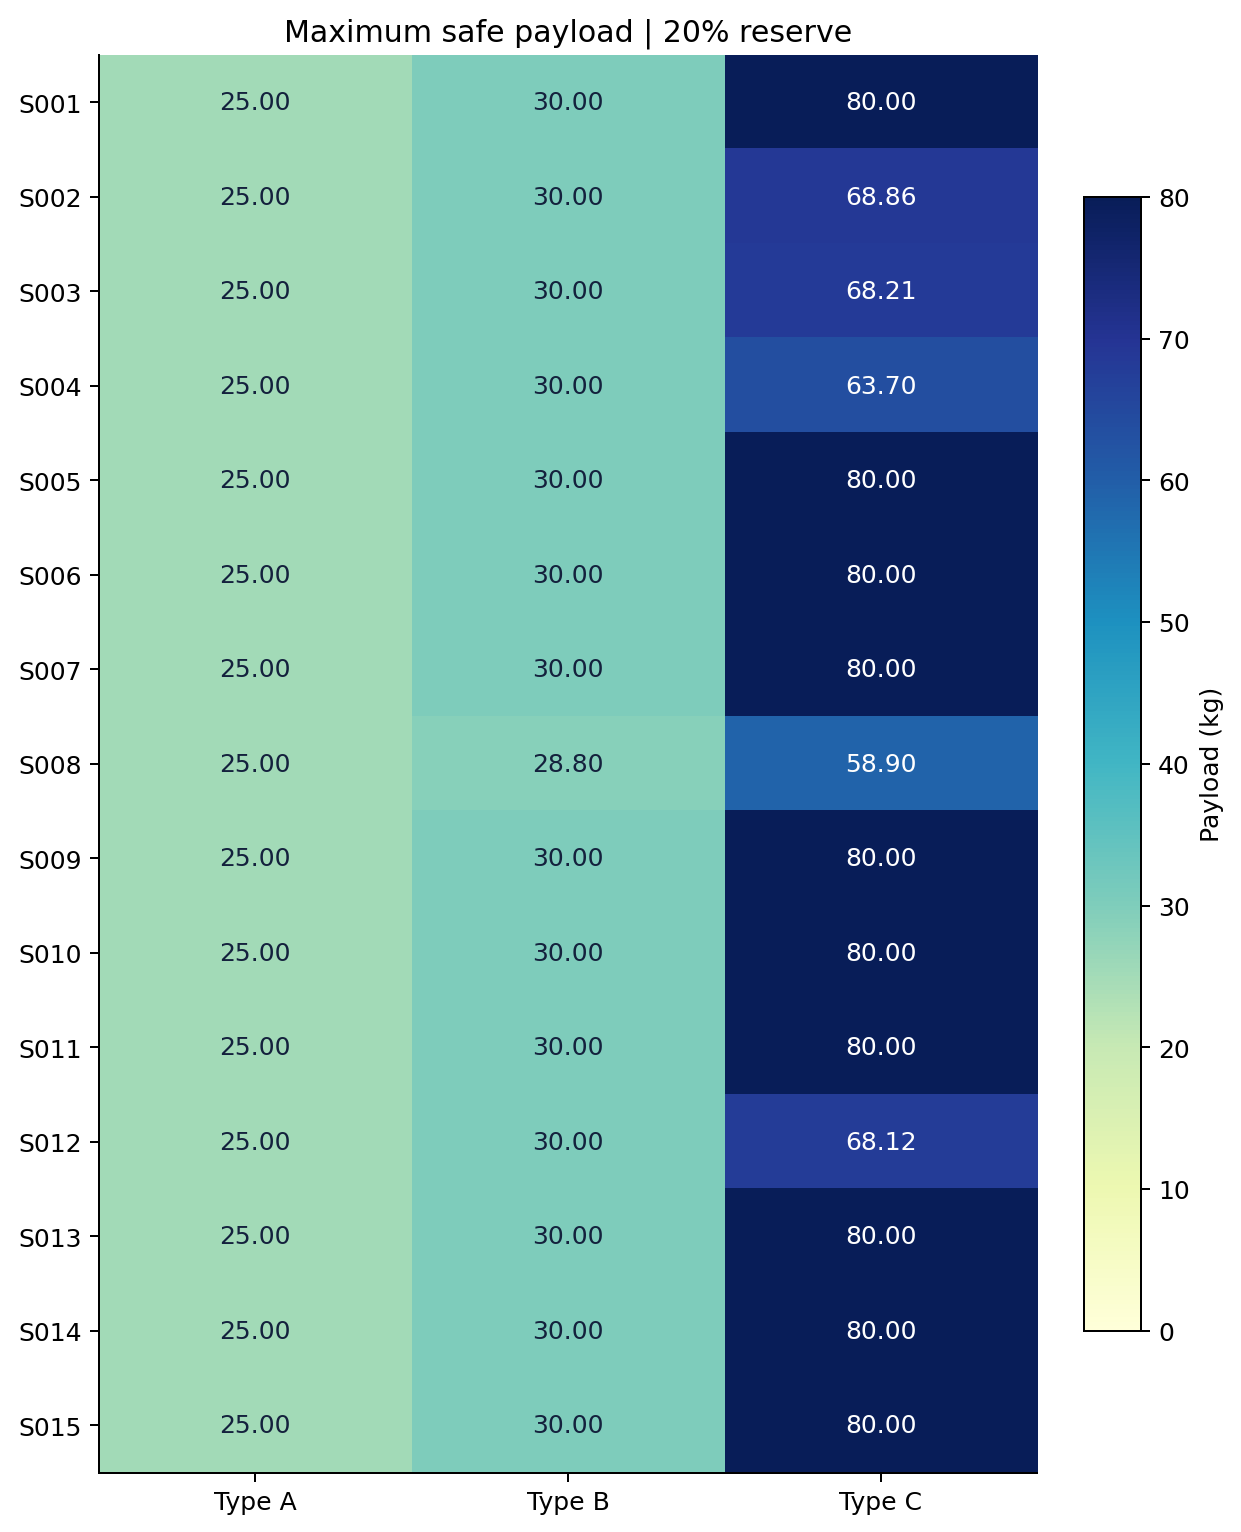
\includegraphics[width=0.72\textwidth]{safe_payload_heatmap.png}
  \caption{20\%返航安全余量下15个服务区与三类机型的最大安全载荷。}
  \label{fig:q1_safe_payload_heatmap}
\end{figure}

\subsection{可行批型与组批模型}

对服务区 $i$ 的任意非空货箱子集 $S\subseteq\mathcal B_i$，若机型 $m$ 同时满足
\[
\sum_{b\in S}\mu_b\le Q_m,
\qquad
\sum_{b\in S}\nu_b\le V_m,
\]
以及
\[
E_{im}\left(\sum_{b\in S}\mu_b\right)
\le(1-\alpha_m)E_m,
\]
则 $(m,S)$ 为可行批型。

定义二元变量 $y_p$ 表示是否选择批型 $p$。每个货箱必须恰好配送一次：
\[
\sum_{p:b\in p}y_p=1.
\]
采用词典序目标：
\[
\boxed{
\min_{\rm lex}(N,E,T^{sum})
}.
\]
即首先最少架次，其次在最少架次条件下降低总能耗，最后缩短累计作业时间。

\subsection{精确求解与交叉验证}

Q1分别建立原始箱级MILP、对称压缩MILP和剩余需求状态DP。原始箱级模型直接枚举原始箱号子集；压缩MILP消除同区同类等价箱号对称；DP以剩余需求向量递推。15个服务区的三种精确方法得到相同词典序目标，因此最终结果不是单一求解器的一次输出。

\begin{table}[H]
\centering
\caption{Q1三种精确方法的交叉验证}
\begin{tabular}{lll}
\toprule
方法 & 主要作用 & 结果\\
\midrule
原始箱级MILP & 原问题精确基准 & 与另外两种方法一致\\
对称压缩MILP & 主精确复现 & 与箱级MILP一致\\
动态规划DP & 独立状态递推与Pareto枚举 & 与MILP一致\\
\bottomrule
\end{tabular}
\end{table}

\subsection{18架次下界与正式主方案}

三类机型中额定载荷最大为80 kg。S001总需求质量154 kg，S002和S003均为81 kg，因此这三个服务区至少各需2架次；其余12个服务区至少各需1架次。于是
\[
N\ge2+2+2+12=18.
\]
精确求解找到满足全部质量、体积与能源条件的18架次方案，因此
\[
\boxed{N^*=18}.
\]

固定18架次后继续最小化总能耗和累计作业时间，得到
\[
\boxed{
N=18,\quad
E=59.131296\ {\rm kWh},\quad
T^{sum}=546.266929\ {\rm min}
}.
\]
机型构成为
\[
A/B/C=0/9/9.
\]

\subsection{强基线与多目标权衡}

为了验证达到18架次后机型和箱组仍具有优化价值，正文优先与强基线比较。全C型精确方案同样为18架次，但能耗约为73.934908 kWh；每个服务区限定单一机型的精确策略约为63.068749 kWh；较强FFD类基线约为64.250537 kWh，而逐架次混合机型精确方案为59.131296 kWh。因此，相同架次数下，精确混合选型仍有明显节能价值。

完整不同Pareto目标向量只有两个：
\[
(18,\ 59.131296,\ 546.266929)
\]
和
\[
(19,\ 59.033942,\ 573.999623).
\]
增加1个架次可节省约0.097354 kWh，但累计作业时间增加约27.733 min，因此
\[
\boxed{\text{最少架次}\neq\text{最低能耗}}.
\]

\begin{figure}[H]
  \centering
  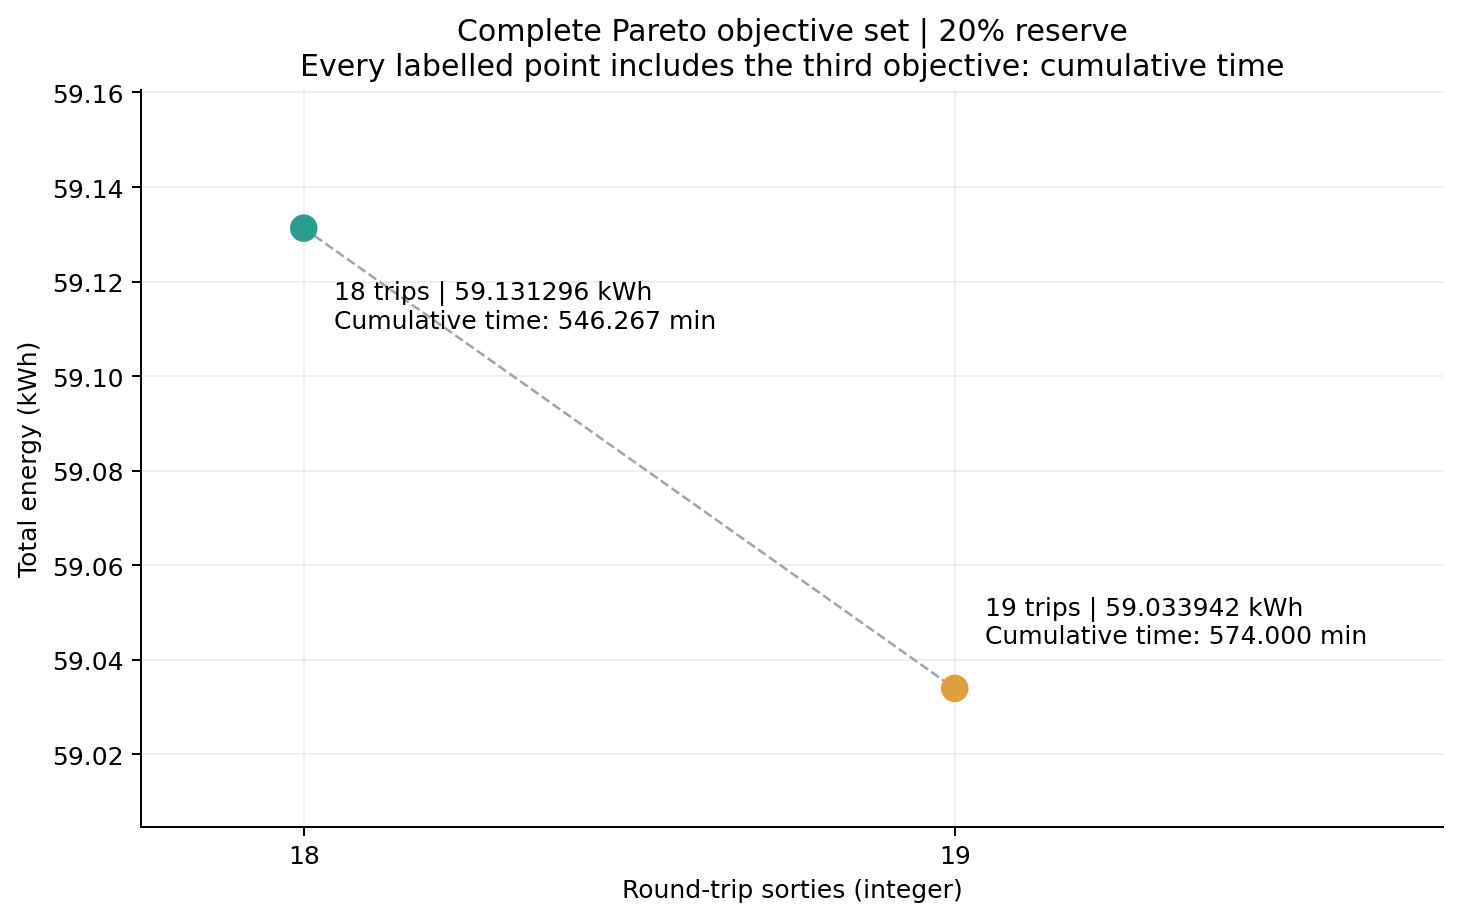
\includegraphics[width=0.78\textwidth]{pareto_front.png}
  \caption{问题一完整离散Pareto目标集合。18架次方案首先达到最少架次数，19架次方案进一步降低少量能耗，但累计作业时间增加。}
  \label{fig:q1_pareto}
\end{figure}

\subsection{安全余量敏感性}

对所有满足额定质量与体积条件的候选批型定义
\[
\rho_p=1-\frac{E_p}{E_m},
\]
则统一安全余量 $\alpha$ 下有
\[
p\text{可行}\iff\alpha\le\rho_p.
\]
完整分析得到569个不同候选事件，其中8个事件会改变全局最少架次数。

\begin{table}[H]
\centering
\caption{统一安全余量引起的主要架次数临界事件}
\begin{tabular}{lcrr}
\toprule
临界余量/\% & 服务区 & 阈值处架次 & 严格右侧\\
\midrule
23.088350 & S004 & 18 & 19\\
27.049854 & S008 & 19 & 20\\
33.625809 & S008 & 20 & 21\\
33.896918 & S003 & 21 & 22\\
34.373532 & S004 & 22 & 23\\
34.391873 & S002 & 23 & 24\\
34.777897 & S008 & 24 & 25\\
35.267807 & S008 & 25 & 不可行\\
\bottomrule
\end{tabular}
\end{table}

当安全余量严格超过约35.2678\%时，S008的一只14 kg饮用水箱即使单独配送，也无法由任一机型完成安全往返；由于货箱不可拆，整个任务直接失去可行解。由此可见，连续安全要求会通过不可拆箱约束转化为离散架次数跃迁。

\begin{figure}[H]
  \centering
  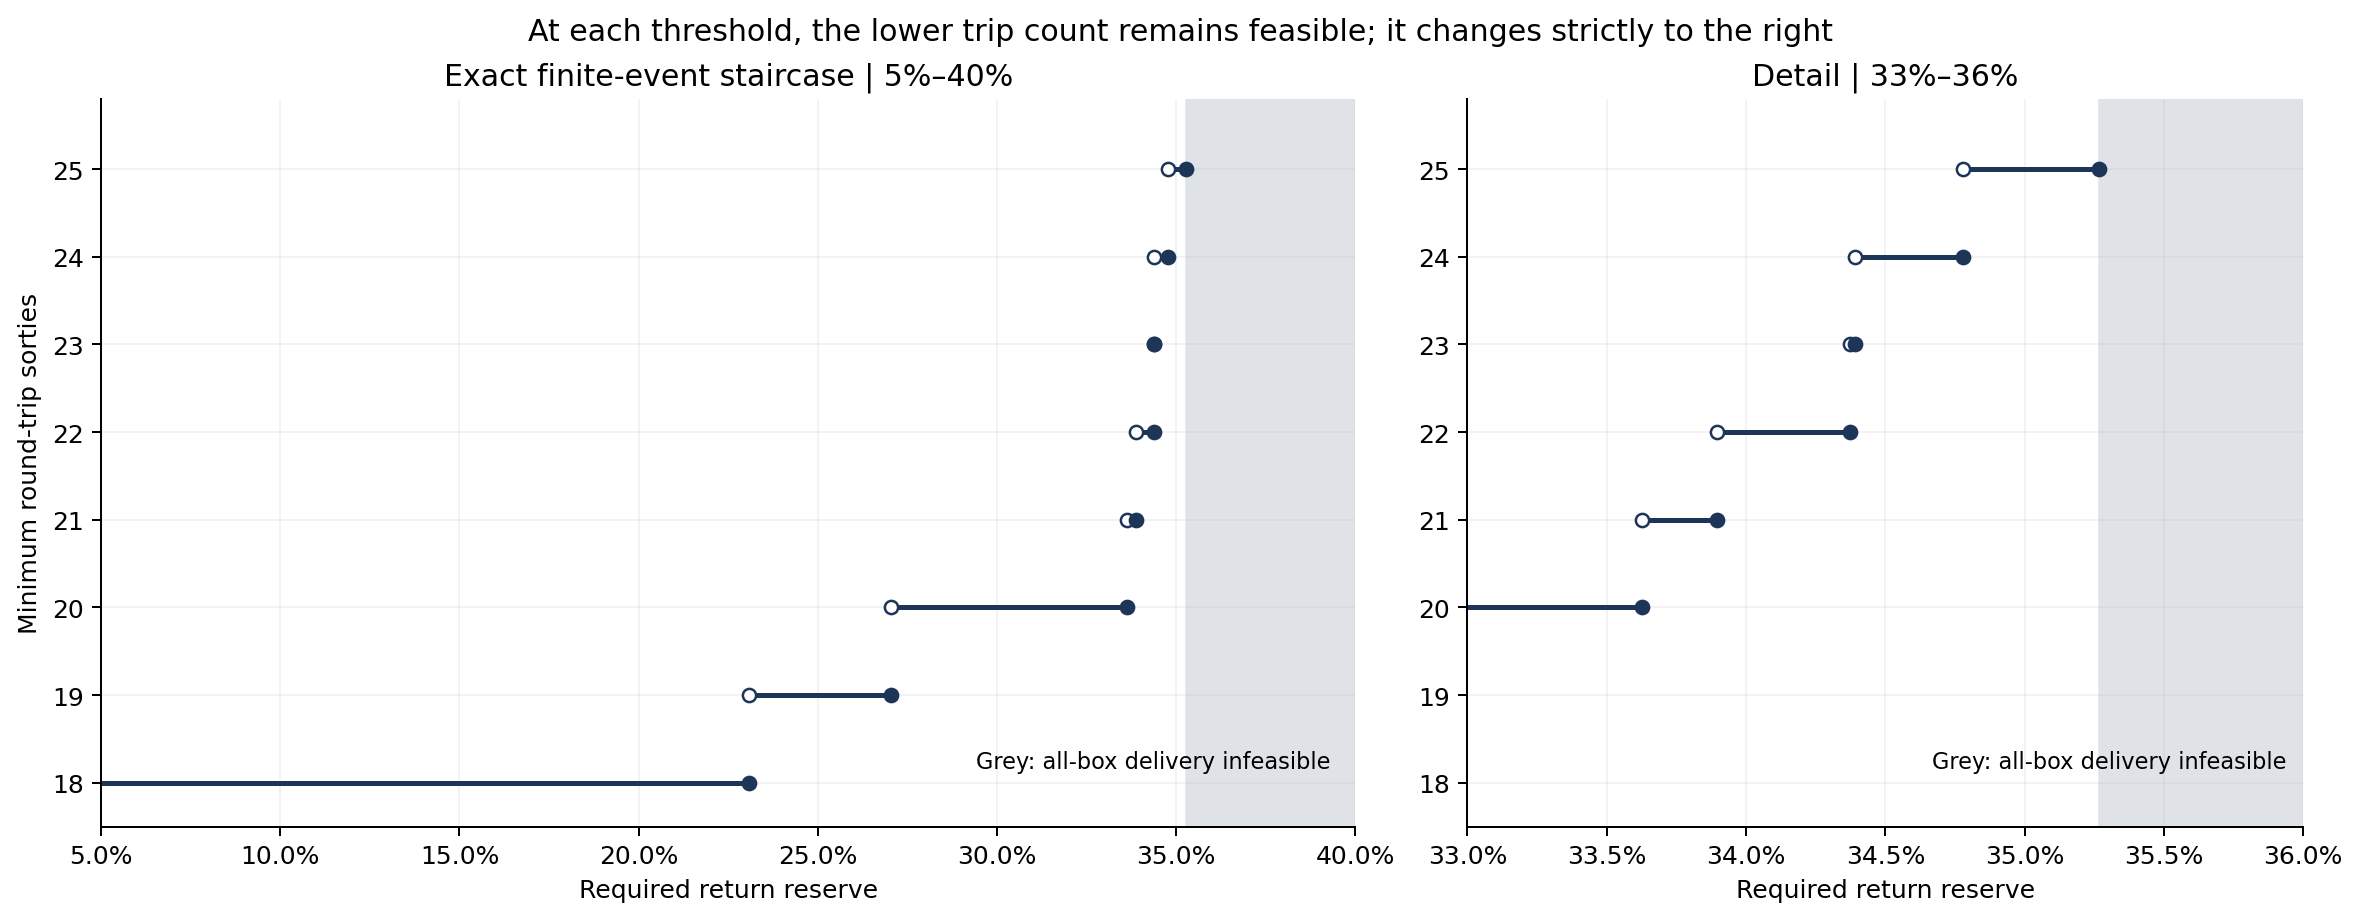
\includegraphics[width=0.95\textwidth]{reserve_vs_min_sorties.png}
  \caption{返航安全余量变化引起的最少架次数阶梯跃迁。连续安全参数通过不可拆货箱组批转化为离散结构变化。}
  \label{fig:q1_reserve_sorties}
\end{figure}

\begin{figure}[H]
  \centering
  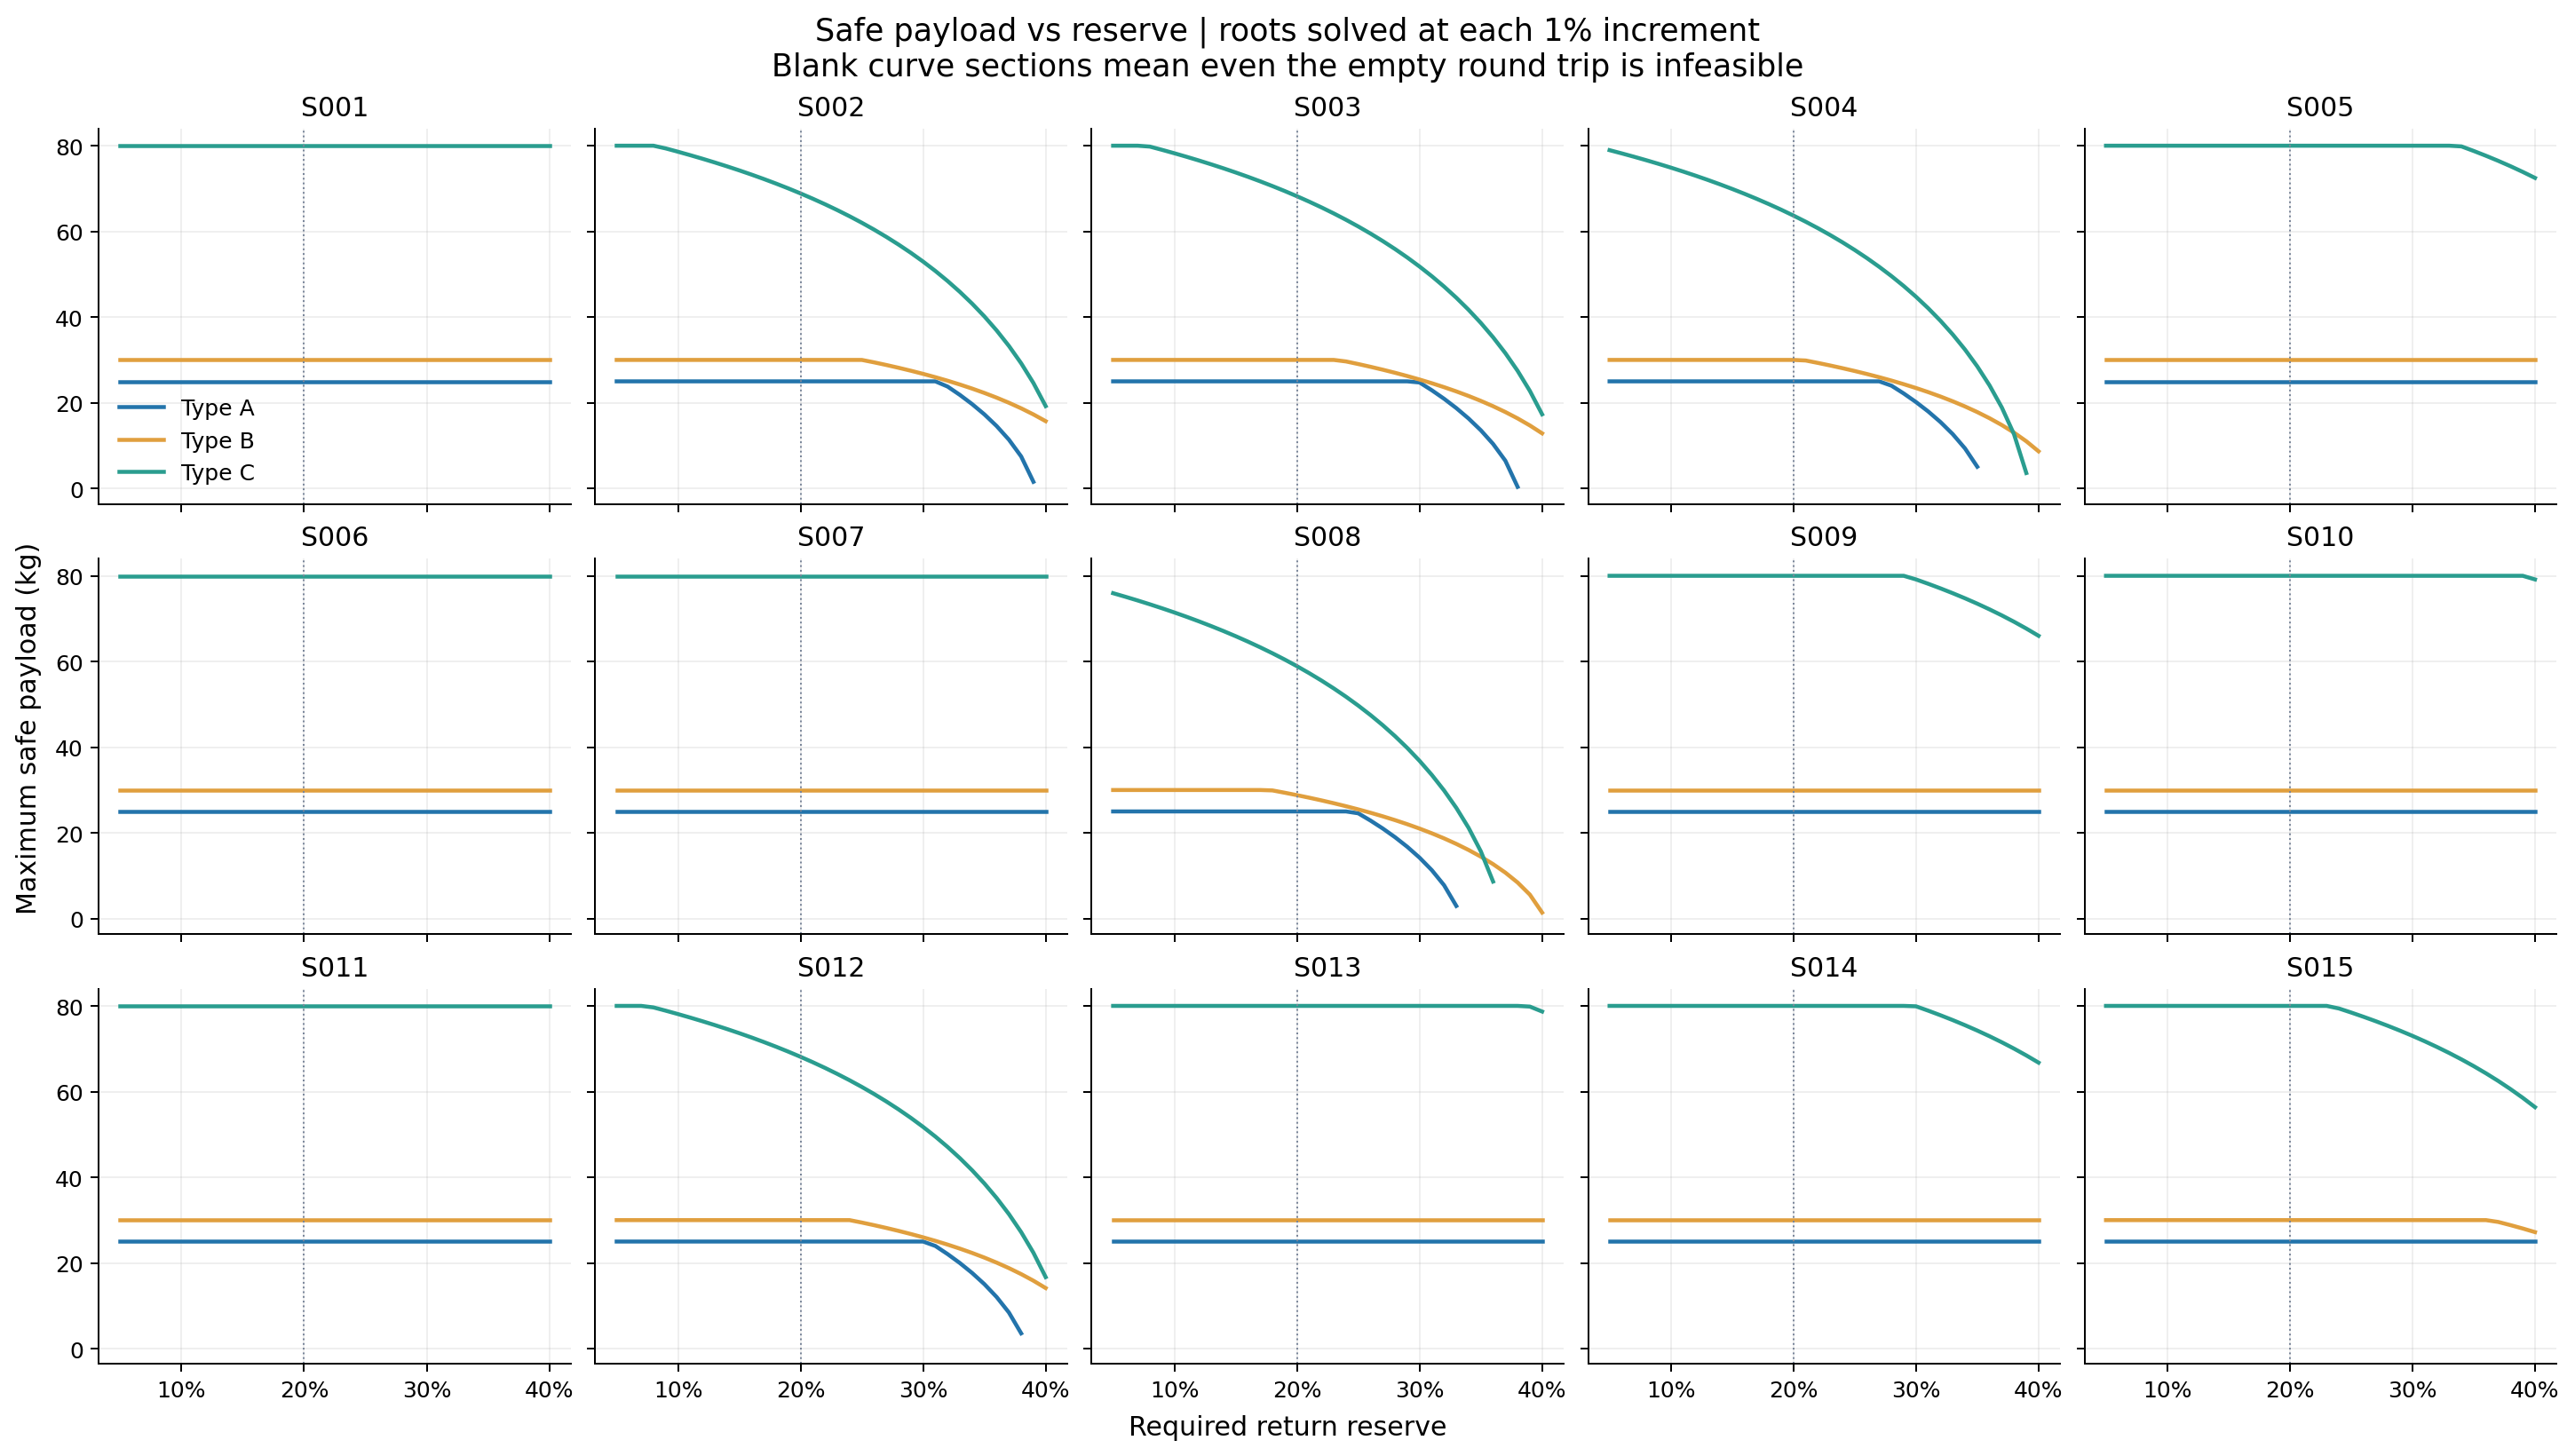
\includegraphics[width=0.98\textwidth]{reserve_vs_safe_payload.png}
  \caption{不同返航安全余量下各服务区三类机型最大安全载荷的变化。该图用于解释架次数临界事件产生的物理来源。}
  \label{fig:q1_reserve_payload}
\end{figure}

% ============================================================
\section{问题二：异构多架次运输与共享电池联合调度}
\label{sec:q2}

\subsection{从单架次可行到系统级可执行}

Q1中一个运输任务只要自身满足物理约束即可视为可行；Q2中任务需要由有限实体无人机和共享电池真实执行。飞机返航并不意味着原电池已经恢复，因此
\[
\boxed{
\text{单架次物理可行}
\not\Rightarrow
\text{完整时间表可执行}
}.
\]

Q2需要同时决定货箱组批、访问路线、机型、实体飞机、电池以及任务开始时刻。

\begin{figure}[H]
  \centering
  \resizebox{0.95\textwidth}{!}{\QTwoFigFramework}
  \caption{问题二从运输任务构造到飞机--电池联合调度及上下界认证的整体框架。可行上界路线负责构造真实可执行时间表，下界路线负责量化当前方案距离理论最优的确定性区间。}
  \label{fig:q2_framework_v7}
\end{figure}

\subsection{运输任务与双资源占用}

第3章统一任务表示仍写为
\[
r=(g_r,\mathcal B_r,\pi_r),
\]
并已计算完整作业时长 $p_r$、能耗 $e_r$、送达偏移 $\delta_{rb}$ 和返航SOC。

设任务在 $s_r$ 开始准备。实体无人机占用区间为
\[
I_r^U=[s_r,s_r+p_r),
\]
若返航后的充电恢复时间为 $c_r$，则电池占用区间为
\[
I_r^B=[s_r,s_r+p_r+c_r).
\]
因此
\[
\boxed{I_r^U\neq I_r^B}.
\]

\begin{figure}[H]
  \centering
  \resizebox{0.88\textwidth}{!}{\QTwoFigOccupancy}
  \caption{单个运输任务对实体无人机和共享电池的不同占用区间。运输无人机返航后即可释放，而原电池仍需继续占用至充电恢复完成。}
  \label{fig:q2_resource_occupancy_v7}
\end{figure}

\subsection{箱级时限与词典序目标}

若箱子 $b$ 由任务 $r$ 运输，则实际送达时刻为
\[
C_b=s_r+\delta_{rb}.
\]
迟到量与加权迟到为
\[
L_b=\max(0,C_b-d_b),
\qquad
L_w=\sum_b\omega_bL_b.
\]
Q2采用词典序目标：
\[
\boxed{
\min_{\rm lex}(L_w,T_{\max},E,N)
}.
\]
首先保证救援物资不迟到，再在零迟到最优面上最小化所有运输任务最后返航时间。

\subsection{联合调度模型与求解框架}

定义任务选择变量、实体飞机指派变量和电池指派变量，分别保证每个货箱恰好覆盖一次、每个已选任务由唯一兼容实体飞机和唯一兼容电池执行。使用同一飞机的任务区间 $I_r^U$ 不得重叠，使用同一电池的任务区间 $I_r^B$ 不得重叠。

完整组合空间同时具有组批、路线、机型和排程耦合，其资源占用与并行调度结构可由经典调度框架刻画\cite{pinedo2016scheduling}。因此采用“高质量可行上界+全局有效下界”的双路线：上界侧通过问题特定的破坏--修复、完整物理重建和事件排程寻找真实可执行方案；下界侧通过任务列松弛、完整定价和互补分支构造证书。大规模列式整数规划中的列生成与branch-and-price思想参见\cite{barnhart1998branchprice}。

\begin{figure}[H]
  \centering
  \resizebox{0.88\textwidth}{!}{\QTwoFigUpperSearch}
  \caption{问题二高质量可行上界搜索与完整资源重放闭环。候选方案只有通过真实飞机、电池、充电恢复和箱级时限重放后，才进入正式可行上界。}
  \label{fig:q2_upper_search_v7}
\end{figure}

\subsection{23架次正式主方案}

第一层加权迟到非负，而正式方案达到
\[
L_w=0,
\]
因此
\[
\boxed{L_w^*=0}.
\]

当前正式主方案包含23个运输架次，
\[
A/B/C=11/6/6,
\]
使用8架实体运输无人机和14组共享电池。最后返航时间为
\[
\boxed{
T_{\max}=5693.231489\ {\rm s}
=94.887191\ {\rm min}
},
\]
总运输能耗为
\[
\boxed{
E=66.214460\ {\rm kWh}
}.
\]
最紧硬截止余量约为202.096 s，最低返航SOC为20.097383\%。

\begin{table}[H]
\centering
\caption{Q2正式主方案主要指标}
\begin{tabular}{lr}
\toprule
指标 & 结果\\
\midrule
加权迟到 & 0\\
运输架次 & 23\\
A/B/C架次 & 11/6/6\\
最后返航时间/s & 5693.231489\\
总运输能耗/kWh & 66.214460\\
实体运输机 & 8\\
共享电池 & 14\\
最紧硬截止余量/s & 202.096058\\
最低返航SOC & 20.097383\%\\
\bottomrule
\end{tabular}
\end{table}

\begin{figure}[H]
  \centering
  \resizebox{0.86\textwidth}{!}{\QTwoFigRouteMap}
  \caption{问题二V7正式23架次方案的空间路线与机型结构。全部路线来自正式incumbent replay；空间几何描述任务构成，资源可执行性由飞机--电池联合甘特图进一步验证。}
  \label{fig:q2_route_map_v7}
\end{figure}

\begin{figure}[H]
  \centering
  \resizebox{0.98\textwidth}{!}{\QTwoFigGantt}
  \caption{问题二V7正式23架次方案的飞机--电池双资源联合甘特图。上图给出8架实体运输无人机的任务链，下图给出14组共享电池的任务占用与充电恢复；虚线对应正式makespan $5693.231489$ s（$94.887$ min）。}
  \label{fig:q2_gantt_v7}
\end{figure}

\subsection{固定B型任务结构下的离散瓶颈}

当前6个B型任务完整作业时间总和为
\[
11133.182841\ {\rm s}.
\]
2架B型飞机的平均负载下界为
\[
5566.591421\ {\rm s},
\]
但6个不可拆任务不能连续均分。对固定B型任务进行精确两机分配，得到更强下界
\[
\boxed{
5693.231489\ {\rm s}
},
\]
而当前时间表恰好达到该值。因此，在保持当前6个B型任务的箱组、机型和路线不变时，仅重新排序已经不能继续缩短当前工期。进一步改善必须改变跨任务货箱、机型或访问结构。该结论仅适用于固定B型任务结构，并非原Q2的全局makespan下界。

\begin{figure}[H]
  \centering
  \resizebox{0.86\textwidth}{!}{\QTwoFigBBottleneck}
  \caption{固定B型任务结构下的两机离散负载瓶颈。连续平均负载下界为$5566.591421$ s，而考虑6个不可拆任务的精确两机分区后，下界提高至$5693.231489$ s；当前U06任务链恰好达到该值。该结论仅针对固定B型任务结构。}
  \label{fig:q2_B_bottleneck_v7}
\end{figure}

\subsection{22架次可行见证与目标冲突}

进一步构造出一份真实可执行22架次方案：
\[
A/B/C=11/4/7,
\]
\[
T_{\max}=7767.058323\ {\rm s},
\qquad
E=66.323024\ {\rm kWh},
\qquad
L_w=0.
\]
因此23架次不是最少可行架次数。但当前22架次见证的工期比23架次主方案长约34.564 min，说明
\[
\boxed{
\text{更少架次}
\not\Rightarrow
\text{更短系统工期}
}.
\]
这里的7767.058 s只是一个可行见证，不是所有22架次方案的下界。

\begin{figure}[H]
  \centering
  \resizebox{0.78\textwidth}{!}{\QTwoFigTwentyTwoTwentyThree}
  \caption{22架次可行见证与23架次V7正式方案的工期--能耗对照。22架次点只证明“22架次可行”，不代表22架次条件下的最优工期，因此不能据此推广为所有22架次方案均更慢。}
  \label{fig:q2_22_23_v7}
\end{figure}

\subsection{全局有效下界与认证区间}

仅搜索不到更好方案不能证明当前方案接近全局最优。为此，将完整运输任务作为列构造set-partitioning松弛，并通过完整定价和互补分支覆盖得到全局有效下界。

当前正式Q2证据版本为 Q2-EVIDENCE-V7-FOCUSED。最终得到
\[
\boxed{
LB=5433.956428\ {\rm s}
}
\]
以及有理上界
\[
\boxed{
UB=5693.231490\ {\rm s}
}.
\]
因此
\[
\boxed{
5433.956428\le T^*\le5693.231490
}.
\]
区间宽度为
\[
259.275062\ {\rm s},
\]
以上界为分母的证据间隙为
\[
\boxed{
\frac{UB-LB}{UB}=4.5541\%
}.
\]

最终覆盖包含809个互补分支与810份叶证书，对全部叶证书重新进行2430次完整机型定价，审计失败为0。上下界尚未闭合，因此不能宣称5693.231489 s已证明为全局最优。

\begin{figure}[H]
  \centering
  \resizebox{0.80\textwidth}{!}{\QTwoFigInterval}
  \caption{问题二V7确定性完成时间认证区间。在零加权迟到最优面上，原问题最优makespan满足$5433.956428\le T^*\le5693.231490$ s，UB归一化证据间隙为$4.5541\%$；由于区间尚未闭合，本文不宣称makespan全局最优。}
  \label{fig:q2_interval_v7}
\end{figure}

\subsection{补充搜索与计算证据}

围绕当前关键任务进行了330个定向局部邻域重构，未发现严格改善上界；另有一个限时模型保持未知，不将其解释为不可行。更大的跨资源链6/7任务有限邻域同样未产生工期改善。这些结果仅支持局部稳定性，不替代全局证明。

针对证明阶段的pricing kernel，在24个固定真实定价输入上，支配强化将各组中位耗时之和由6.323099 s降至2.026581 s，比值为3.1201；累计生成标签由5,706,982降至2,061,175，减少63.88\%，且24个输入的最小约化成本全部保持一致。随后完整重定价810份证书、2430次调用后原下界仍有效。该3.1201倍仅表示固定pricing输入的合计中位耗时比，不表示整个Q2求解器提速3.12倍。

\begin{figure}[H]
  \centering
  \resizebox{0.78\textwidth}{!}{\QTwoFigPricing}
  \caption{问题二定价器支配强化的受控配对实验。24组固定真实定价输入的各组中位耗时之和由$6.323099$ s降至$2.026581$ s，生成标签减少$63.88\%$，且24/24输入的最小约化成本保持一致。图中$3.1201\times$仅表示该受控pricing实验的中位耗时之和比，不代表整个Q2求解器获得同等加速。}
  \label{fig:q2_pricing_v7}
\end{figure}

% ============================================================
\section{问题三：连续通信约束下的运输--中继联合优化}
\label{sec:q3}

\subsection{从运输可执行到全过程通信可用}

Q2运输时间表仍隐含“运输无人机全过程通信可用”的条件。山区地形可能使无人机在爬升、巡航、下降或返回途中出现通信遮挡，因此
\[
\boxed{
\text{运输计划可执行}
\not\Rightarrow
\text{运输全过程通信可用}
}.
\]

设运输无人机、中继无人机和地面站分别为 $U,R,G$。直连可用时优先采用 $U\leftrightarrow G$；直连失效时允许一次中继
\[
U\leftrightarrow R\leftrightarrow G.
\]
中继无人机同样需要起飞、到位、服务、返航和能源恢复，因此Q3本质上是运输轨迹、连续通信和中继资源时序的联合问题。

\figplaceholder{图6-1占位：从运输可执行到连续通信保障的模型升级。}

\subsection{链路预算与连续通信状态}

无人机辅助无线通信具有高度可控的三维移动性，同时受到视距传播、能量与时空资源耦合约束\cite{zeng2016uavcom,zeng2019sky}。自由空间传播损耗计算采用标准链路预算口径\cite{iturp525}。三类链路允许损耗上限为
\[
L_{UG}^{\max}=122\ {\rm dB},\qquad
L_{UR}^{\max}=116\ {\rm dB},\qquad
L_{RG}^{\max}=126\ {\rm dB}.
\]
定义链路余量
\[
M_{ab}(t)=L_{ab}^{\max}-L_{ab}(t).
\]
若考虑额外统一传播损耗 $\Delta$，则链路需满足
\[
M_{ab}(t)\ge\Delta.
\]
通信可行同时要求链路预算满足且传播路径未被地形阻挡。

对运输任务 $r$，无人机位置随时间连续变化，记为 $\mathbf x_r(t)$。定义直连不可用时间集合
\[
\mathcal W_r
=
\{t\in\mathcal T_r:\chi_{UG}(t)=0\}
=
\bigcup_{\ell=1}^{n_r}[a_{r\ell},b_{r\ell}].
\]
每个区间对应一项真实中继服务需求。本文不以固定步长采样替代连续条件，而根据轨迹分段、传播几何和通信状态变化构造区间并检查临界端点。

\figplaceholder{图6-2占位：代表运输任务沿时间轴的直连状态与中继需求区间。}

\subsection{中继转场高度与候选域}

候选悬停位置记为 $p$，其地面高程和悬停海拔分别为 $z_g(p)$ 与 $z_p$。早期实现把中继悬停海拔限制在“调度中心至候选点沿线最高地形+50 m”之下，这会额外缩小题面允许的悬停高度空间。当前模型只对中继往返转场采用
\[
\boxed{
H_R(p)=
\max\left\{
\max_{c\in\mathcal C(O01,p)}Z(c)+50,\;
z_p,\;
z_{O01}
\right\}
}
\]
作为巡航海拔：既满足地形净空，又能够到达给定悬停端点。所有爬升、下降、水平飞行、建链、悬停、返航和充电代价均重新计算；普通运输航段仍保持“经过像元最高地形+50 m”的原规则。悬停离地高度不超过300 m。

这个修订改变的是中继候选域而不是通信判据，因此旧的5755候选位置有限域证书不能继续作为当前V6的中继架次数下界。

\figplaceholder{图6-3占位：中继转场高度、悬停高度与地形净空的关系。}

\subsection{运输--通信联合模型与求解闭环}

对每个运输任务，先从真实三维轨迹构造直连不可用的连续区间及临界端点，再计算各中继候选在完整区间内的接入与回传共同可用性。优化变量同时覆盖运输开始时刻、中继位置与高度、服务窗口、中继实体、能源组件以及通信提供方切换。

在保持零加权迟到、20\%返航SOC和至少30 s硬截止缓冲的前提下，主目标为最小化
\[
T_{\max}^{joint}=\max\{T_{\max}^{U},T_{\max}^{R}\}.
\]
求解采用“角色感知位置/高度候选--完整几何重建--联合整数排程--固定离散结构连续时间精修--独立验证”的闭环。廉价采样仅用于候选排序，任何被接受的方案都重新检查完整区间和临界端点。

\figplaceholder{图6-4占位：Q3候选生成、联合排程、连续精修和独立验证流程。}

\subsection{正式运输--通信联合方案}

正式 \texttt{time} 方案包含
\[
\boxed{23\text{个运输架次}+4\text{个中继架次}}.
\]
运输部分使用8架实体运输无人机和14组运输电池；中继部分实际使用2架中继无人机和3组中继能源组件。

联合最后返航时间为
\[
\boxed{
T_{\max}^{joint}=5836.969929\ {\rm s}
=97.283\ {\rm min}
},
\]
运输能耗为
\[
66.251280\ {\rm kWh},
\]
中继能耗为
\[
2.688136\ {\rm kWh},
\]
总能耗为
\[
\boxed{68.939416\ {\rm kWh}}.
\]
80个货箱均完成唯一交付，加权迟到和硬迟到均为0；最小硬截止余量为360.866938 s，最低运输返航SOC为20.097383\%。

\begin{table}[H]
\centering
\caption{Q3 V6正式联合方案主要指标}
\begin{tabular}{lr}
\toprule
指标 & 结果\\
\midrule
运输架次 & 23\\
中继架次 & 4\\
联合最后返航/s & 5836.969929\\
运输能耗/kWh & 66.251280\\
中继能耗/kWh & 2.688136\\
总能耗/kWh & 68.939416\\
加权迟到 & 0\\
最小硬截止余量/s & 360.866938\\
最低运输返航SOC & 20.097383\%\\
\bottomrule
\end{tabular}
\end{table}

\figplaceholder[7.0cm]{图6-5占位：V6运输轨迹、四个中继悬停位置与实际通信保障关系。}

\subsection{通信切换驱动的关键同步链}

V6相对于上一版在相同物理、通信和库存模型下进一步缩短87.997560 s。对最后关键C型运输任务进行依赖链分析可发现，主要收益并非来自缩短飞行距离，而来自改变通信保障切换时刻。

上一版该任务在相对开始时刻956.973974 s后必须依赖西侧中继；V6通过调整中继布局，使前段保障延长到1039.150288 s，交接需求推迟
\[
\boxed{82.176314\ {\rm s}}.
\]
同时，西侧中继可服务时刻提前
\[
\boxed{5.821245\ {\rm s}}.
\]
二者合计约87.997559 s，与关键运输任务允许提前的时间基本一致。这说明在运输--通信联合系统中，中继位置不仅决定“能否覆盖”，还会通过提供方切换边界改变运输任务的最早可执行时刻。

\figplaceholder{图6-6占位：北侧保障延长--西侧中继提前就绪--关键C型任务提前开始的同步链。}

\subsection{连续通信完整验证}

正式V6方案对真实运输时序重新生成通信几何。主验证器完成17,756项物理、资源、区间与端点检查，失败0；另一路独立时空点过程生成36,672个包含边界的核验点，未发现断链。方案包含700份完整区间证书和1,238份临界端点证书。

因此当前证据支持“保存的V6方案在既定数值模型下完整可行”，但不把验证计数解释为实飞次数，也不据此宣称原Q3全局最优。

\figplaceholder{图6-7占位：代表运输任务的Direct/Relay提供方切换与临界端点。}

\subsection{时间--能耗与通信裕度权衡}

除最快主方案外，还保留两个具有不同目标偏好的完整可行方案。

\begin{table}[H]
\centering
\caption{Q3 V6时间、能耗与通信裕度方案}
\begin{tabular}{lrrr}
\toprule
方案 & 额外损耗/dB & 联合工期/s & 总能耗/kWh\\
\midrule
time & 0 & 5836.969929 & 68.939416\\
energy & 0 & 5911.548135 & 68.735791\\
robust025 & 0.25 & 5866.140527 & 69.031751\\
\bottomrule
\end{tabular}
\end{table}

节能方案比最快方案晚74.578205 s，但少耗0.203625 kWh；额外0.25 dB方案比最快方案晚29.170597 s。0.5 dB和1 dB在已测试固定布局中出现未覆盖需求，因此未作为可行方案发布；这不能推广为整个连续选址空间的最大通信裕度。

\figplaceholder{图6-8占位：V6最快、节能与+0.25 dB保障方案的离散权衡。}

\subsection{当前最优性边界}

在固定同一23个运输模式、去掉通信与中继约束后，运输排程可达到约5693.231489 s；与V6最快方案仍相差约143.738440 s。这个差值只说明固定运输结构下通信与中继时序仍有潜在优化空间，不是Q3原问题的严格下界。

因此当前正式结论是：V6是经过全精度验证的当前最优已知联合方案；不宣称全局最优，也不继承旧候选域的4中继下界或旧0.50/0.55 dB鲁棒结论。

% ============================================================
\section{问题四：独立任务分组下的异构资源配置与池化损失}
\label{sec:q4}

\subsection{问题分析与建模目标}

前三问均在统一资源池下组织任务：同型号运输无人机、电池以及中继资源可以在不同服务区任务之间按时间先后重复使用。问题四进一步要求将15个服务区划分为若干相互独立的任务组，各组需要依靠本组配置独立完成既定救援任务，不允许跨组临时借用实体资源。因而问题四并不是重新求解一遍问题三，而是研究一个更具体的系统问题：
\[
\boxed{
\text{当既定联合救援计划被组织边界切开后，原有资源复用能力会损失多少？}
}
\]

为保证跨问题口径一致，本文严格继承问题三当前正式的
\texttt{Q3-BOTTLENECK-V6/time} 方案，冻结货箱组批、运输机型、访问顺序、绝对开始时刻、中继位置、服务窗口以及实际通信保障关系，只改变服务区所属任务组。换言之，第七章评价的是“既定V6预案在独立组织条件下需要配置多少资源”，而不是允许重新设计Q3路线和日程后的理论最小资源数。

据此，将问题四的求解过程概括为
\[
\boxed{
\text{冻结V6日程}
\rightarrow
\text{构造不可拆任务块}
\rightarrow
\text{完整枚举分组}
\rightarrow
\text{计算组内资源峰值}
\rightarrow
\text{计算缺口与均衡性}
\rightarrow
\text{交叉验证}
}.
\]
这一处理把“区域怎么分”和“每组究竟要多少设备”分成两个清晰层次：前者是离散分区问题，后者是在固定时间表上的精确资源配置问题。

\subsection{V6固定任务与资源占用表示}

记冻结后的运输任务集合和逻辑中继任务集合分别为
\[
\mathcal J^T,\qquad \mathcal J^R,
\]
总固定任务集合为
\[
\mathcal J=\mathcal J^T\cup\mathcal J^R.
\]
当前V6日程包含23个运输架次和4个逻辑中继架次。每个任务的空间路径、开始时刻、返航时刻和资源恢复规则均由第6章正式方案给定，第七章不再改变。

资源类型集合写为
\[
\mathcal P=
\{U_A,U_B,U_C,B_A,B_B,B_C,U_R,K_R\},
\]
分别表示A/B/C型运输无人机、A/B/C型运输电池、中继无人机和中继能源组件。原始库存向量为
\[
\boxed{
\mathbf I=(4,2,2,6,4,4,2,6)
}.
\]

对于任务 $j$ 使用的资源类型 $p$，将该资源在冻结日程中的占用写成半开区间
\[
I_{jp}=[s_{jp},r_{jp}).
\]
其中运输无人机通常占用至任务返航，运输电池还要继承返航后的恢复时间；中继无人机与中继能源组件同样继承第6章既定的返航和恢复规则。因此同一个任务对不同类型资源的释放时刻可以不同，不能只根据任务返航时间粗略估计资源数量。

半开区间的使用具有实际意义：若一个资源在时刻 $t$ 恰好释放，而另一任务也在 $t$ 开始，则两者允许首尾衔接，不应被误判为资源冲突。

\subsection{不可拆任务块的构造}

\subsubsection{服务区关联关系}

对于每个冻结任务 $j\in\mathcal J$，记其实际关联的服务区集合为 $\mathcal A_j$。运输任务的 $\mathcal A_j$ 由实际访问路径决定；逻辑中继任务的 $\mathcal A_j$ 由V6保存的实际通信保障关系决定。

严格独立执行要求：若两个服务区同时出现在某一冻结任务的关联集合中，则它们不能被拆到不同任务组，否则就必须复制或改写原任务，违背“冻结Q3正式计划”的前提。因此定义服务区关联图
\[
\mathcal G=(\mathcal S,\mathcal E),
\]
若存在任务 $j$ 使得
\[
u,v\in\mathcal A_j,
\]
则在 $u,v$ 之间建立关联边。由于同一任务产生的约束具有传递性，关联图的每个连通分量必须整体进入同一任务组。

\subsubsection{V6日程下的三个不可拆块}

按照当前V6运输与实际中继保障关系，15个服务区最终形成三个连通分量：
\[
B_1=\{S001\},
\]
\[
B_2=
\{S002,S003,S004,S005,S007,S008,S009,S010,S011,S012,S013,S014,S015\},
\]
\[
B_3=\{S006\}.
\]

因此，问题四真正需要划分的并不是15个彼此独立的服务区，而是3个不可拆任务块。这个压缩极大降低了组合规模，同时没有损失任何严格可行分区。

若将3个不可拆块划分为 $K$ 个非空、无标签任务组，则合法分区数为第二类Stirling数 $S(3,K)$。于是
\[
S(3,2)=3,\qquad S(3,3)=1.
\]
严格两组的三个候选分别为
\[
\Pi_2^{(1)}=\{B_1\cup B_2,\ B_3\},
\]
\[
\Pi_2^{(2)}=\{B_1\cup B_3,\ B_2\},
\]
\[
\Pi_2^{(3)}=\{B_1,\ B_2\cup B_3\},
\]
而严格三组只有
\[
\Pi_3=\{B_1,B_2,B_3\}.
\]

因此本问不需要启发式搜索或随机优化，所有合法分区都可以完整枚举。

\subsection{组内最小分类型资源配置模型}

\subsubsection{资源峰值模型}

给定一个候选分区 $\Pi$，记第 $g$ 个任务组包含的冻结任务集合为 $\mathcal J_g$。对于资源类型 $p$，定义时刻 $t$ 的同时占用数量
\[
n_{gp}(t)
=
\sum_{j\in\mathcal J_g}
\mathbf 1\{t\in I_{jp}\}.
\]
则该组独立执行时对资源类型 $p$ 的最小配置数为
\[
\boxed{
N_{gp}^{\min}
=
\max_t n_{gp}(t)
}.
\]

这一式子不是经验估计，而是固定区间条件下的精确最小值。一方面，在达到最大重叠的某个时刻 $t^*$，存在 $N_{gp}^{\min}$ 个任务同时占用该类型资源，因此任何可执行配置都至少需要这么多资源。另一方面，将同类型任务按开始时刻排序，每次优先分配给“最早已经释放”的资源；若当前没有可用资源，再新建一条资源链。由于所有占用均为一维区间，该构造使用的资源数恰等于最大同时重叠数。因此
\[
\boxed{
\text{最大并发峰值}
=
\text{该组该类型资源的精确最小配置}
}.
\]

\subsubsection{独立分组后的总需求与缺口}

分区 $\Pi$ 下，资源类型 $p$ 的总独立配置需求为
\[
D_p(\Pi)
=
\sum_{g\in\Pi}N_{gp}^{\min}.
\]
与原始库存比较，得到分类型资源缺口
\[
G_p(\Pi)
=
\max\{0,D_p(\Pi)-I_p\}.
\]
进一步定义总缺口
\[
G_{\Sigma}(\Pi)=\sum_{p\in\mathcal P}G_p(\Pi),
\]
以及总配置数
\[
D_{\Sigma}(\Pi)=\sum_{p\in\mathcal P}D_p(\Pi).
\]

这里必须保留完整缺口向量
\[
\mathbf G(\Pi)
=
(G_{U_A},G_{U_B},G_{U_C},G_{B_A},G_{B_B},G_{B_C},G_{U_R},G_{K_R}),
\]
因为不同类型资源不可互换。即使设备总数看似充足，也可能因为某一关键型号短缺而无法独立执行。

\subsubsection{工作量均衡指标}

为在前两层资源指标相同时比较任务组的执行负担，记冻结日程中任务 $j$ 从开始至返航的完整执行时长为
\[
\tau_j=t_j^{return}-t_j^{start},
\]
第 $g$ 组工作量定义为
\[
W_g=\sum_{j\in\mathcal J_g}\tau_j.
\]
运输架次与逻辑中继架次均按其完整执行时长计入。设任务组数为 $K$，则
\[
\overline W=\frac{1}{K}\sum_{g=1}^{K}W_g,
\]
工作量变异系数为
\[
\boxed{
CV_W
=
\frac{
\sqrt{\frac{1}{K}\sum_{g=1}^{K}(W_g-\overline W)^2}
}{
\overline W
}
}.
\]

当前程序保存的两组与三组结果分别为
\[
CV_W^{(2)}=0.941761573,
\qquad
CV_W^{(3)}=1.183797501,
\]
与按V6冻结任务逐项重算完全一致。

\subsubsection{词典序评价准则}

救援场景下，首先需要尽量减少因独立执行新增的资源缺口；在缺口相同的情况下，再减少独立配置总量；只有前两层均相同时，才考虑任务工作量均衡。因此采用
\[
\boxed{
\min_{\rm lex}
\left(
G_{\Sigma},
D_{\Sigma},
CV_W,
ID(\Pi)
\right)
}.
\]
最后的规范分区编号 $ID(\Pi)$ 只用于完全同值时稳定复现结果，不参与实际管理含义的解释。

\subsection{完整枚举与求解流程}

由于不可拆块只有3个，本问采用精确完整枚举而非启发式算法。具体步骤如下。

\begin{enumerate}[label=\textbf{步骤\arabic*.},leftmargin=4.5em]
\item 读取Q3 V6 \texttt{time} 正式方案并锁定运输、中继、绝对时刻及资源恢复规则，禁止在Q4求解过程中修改任务。
\item 根据多服务区运输任务与实际中继保障关系建立服务区关联图，求连通分量得到 $B_1,B_2,B_3$ 三个不可拆块。
\item 对 $K=2$ 和 $K=3$ 分别枚举全部无标签非空分区，得到3个和1个候选。
\item 对每个候选分区、每个任务组和每种资源生成事件集合
\[
\mathcal E_{gp}
=
\{(s_{jp},+1),(r_{jp},-1):j\in\mathcal J_g\}.
\]
按时间排序；同一时刻先处理释放事件再处理占用事件，以保持半开区间语义。扫描前缀和即可得到 $N_{gp}^{\min}$。
\item 使用“最早释放优先”的同型资源链重新构造实体分配，并使用独立匹配方法交叉核验，检查峰值结果确实能够被实体资源链实现。
\item 计算 $\mathbf D(\Pi)$、$\mathbf G(\Pi)$、$G_\Sigma$、$D_\Sigma$ 与 $CV_W$，按词典序准则选出正式方案。
\end{enumerate}

若某候选分区共有 $M$ 个资源占用区间，则事件扫描复杂度为
\[
O(M\log M).
\]
本题只需评价4个合法分区，每个分区仅含8种资源，因此求解空间被完整覆盖，不存在随机初值、停止准则或“未搜索到更优”带来的最优性不确定性。

\begin{table}[H]
\centering
\caption{问题四严格模型的完整枚举规模}
\label{tab:q4_enum_size}
\begin{tabular}{cccc}
\toprule
任务组数 $K$ & 不可拆块数 & 无标签合法分区 & 求解方式\\
\midrule
2 & 3 & 3 & 全部枚举并逐分区精确计算资源峰值\\
3 & 3 & 1 & 唯一分区直接精确计算\\
\bottomrule
\end{tabular}
\end{table}

\subsection{严格两组的求解结果}

对 $\Pi_2^{(1)},\Pi_2^{(2)},\Pi_2^{(3)}$ 三个候选全部计算后，词典序准则选择
\[
\boxed{
\Pi_2^*
=
\{\text{除S006外的14个服务区}\}
\mid
\{S006\}
}.
\]
其分类型资源需求为
\[
\boxed{
\mathbf D^{(2)}
=
(4,2,3,6,4,4,2,3)
},
\]
相对原始库存的缺口向量为
\[
\boxed{
\mathbf G^{(2)}
=
(0,0,1,0,0,0,0,0)
}.
\]
因此
\[
\boxed{
D_{\Sigma}^{(2)}=28,\qquad
G_{\Sigma}^{(2)}=1
}.
\]

也就是说，两组能够独立执行所需的唯一新增资源是1架C型运输无人机。这里有一个容易被总量指标掩盖的现象：两组独立配置总需求只有28件，小于原始库存总数30件，但C型运输无人机的需求为3架、库存只有2架，因此系统仍然存在1个刚性缺口。多余的中继能源组件不能替代C型运输无人机，这正是异构资源配置必须按类型计算的原因。

当前选中分区的工作量变异系数为
\[
CV_W^{(2)}=0.941761573.
\]
由于工作量均衡位于词典序第三层，不能为了降低CV而接受更大的资源缺口或更高的独立配置总量。

\subsection{严格三组的求解结果}

三组条件下只有一个严格合法分区：
\[
\boxed{
\Pi_3^*
=
\{S001\}
\mid
\{\text{其余13个服务区}\}
\mid
\{S006\}
}.
\]
其资源需求向量为
\[
\boxed{
\mathbf D^{(3)}
=
(5,2,5,7,4,6,2,3)
},
\]
缺口向量为
\[
\boxed{
\mathbf G^{(3)}
=
(1,0,3,1,0,2,0,0)
}.
\]
因此
\[
\boxed{
D_{\Sigma}^{(3)}=34,\qquad
G_{\Sigma}^{(3)}=7
}.
\]

具体而言，需要新增1架A型运输无人机、3架C型运输无人机、1组A型电池和2组C型电池。三组资源总需求34件仅比库存总数30件多4件，但分类型缺口之和却达到7件。原因是中继能源组件等类型仍有富余，而这些富余不能抵消运输无人机和运输电池的型号短缺，因此
\[
\boxed{
\sum_p\max(0,D_p-I_p)
\neq
\max\left(0,\sum_pD_p-\sum_pI_p\right)
}.
\]
这进一步说明“设备总数差额”不是独立资源配置的有效评价指标。

三组唯一分区的工作量变异系数为
\[
CV_W^{(3)}=1.183797501.
\]

\subsection{资源池化损失的定量解释}

在不进行独立分组时，Q3 V6全局共享日程对8类资源的实际峰值需求为
\[
\mathbf N^{pool}
=
(4,2,2,6,4,4,2,3),
\]
总计27件。独立分组后，同一类型资源无法跨组错峰复用。对资源类型 $p$，定义池化损失
\[
L_p(\Pi)
=
\sum_{g\in\Pi}\max_t n_{gp}(t)
-
\max_t\sum_{g\in\Pi}n_{gp}(t).
\]
由“峰值之和不小于总量峰值”可得
\[
L_p(\Pi)\ge0.
\]

两组正式方案的池化损失向量为
\[
\boxed{
\mathbf L^{(2)}
=
(0,0,1,0,0,0,0,0)
},
\]
三组正式方案为
\[
\boxed{
\mathbf L^{(3)}
=
(1,0,3,1,0,2,0,0)
}.
\]
因此，两组独立执行只破坏了1个C型运输无人机的跨组复用机会；三组独立执行则同时破坏A/C型运输无人机和A/C型电池的错峰复用链。

\begin{table}[H]
\centering
\small
\caption{V6日程下全局共享与独立分组的分类型资源需求}
\label{tab:q4_resource_compare}
\begin{tabular}{lrrrrrr}
\toprule
资源类型 & 原库存 & Q3共享峰值 & K=2需求 & K=2缺口 & K=3需求 & K=3缺口\\
\midrule
A型运输机 & 4 & 4 & 4 & 0 & 5 & 1\\
B型运输机 & 2 & 2 & 2 & 0 & 2 & 0\\
C型运输机 & 2 & 2 & 3 & 1 & 5 & 3\\
A型电池 & 6 & 6 & 6 & 0 & 7 & 1\\
B型电池 & 4 & 4 & 4 & 0 & 4 & 0\\
C型电池 & 4 & 4 & 4 & 0 & 6 & 2\\
中继无人机 & 2 & 2 & 2 & 0 & 2 & 0\\
中继能源组件 & 6 & 3 & 3 & 0 & 3 & 0\\
\midrule
总计 & 30 & 27 & 28 & 1 & 34 & 7\\
\bottomrule
\end{tabular}
\end{table}

从表中可以看到，独立执行增加的并不是所有资源，而是少数位于关键复用链上的瓶颈型号。中继能源组件原库存为6组，而Q3共享、两组独立和三组独立均只需要3组，因此继续增加这类非瓶颈资源并不能修复运输侧的独立执行缺口。

\subsection{跨问题对照：最短联合工期与最省独立配置并不一致}

为检验Q3“最快完成”是否也自然对应Q4“最省独立资源”，进一步保留一份面向Q4的跨问对照候选。正式Q3 \texttt{time} 方案的联合工期和总能耗为
\[
5836.969929\ {\rm s},
\qquad
68.939416\ {\rm kWh},
\]
其严格三组资源缺口为7。

另一个 \texttt{q4\_tradeoff} 候选的联合工期为
\[
5866.140527\ {\rm s},
\]
总能耗为
\[
68.975497\ {\rm kWh},
\]
对应严格三组缺口可降至6。与正式最快方案相比，它牺牲约
\[
29.170597\ {\rm s}
\]
的联合工期并增加约
\[
0.036081\ {\rm kWh}
\]
能耗，换取1个独立配置缺口的减少。

该方案不替代Q3最快主答案，也不替代本节基于Q3 \texttt{time} 的Q4正式答案；它只用于说明
\[
\boxed{
\text{Q3最短联合工期}
\not\Rightarrow
\text{Q4最少独立资源缺口}
}.
\]
这类跨层权衡比简单比较“设备总数”更能反映救援预案在组织方式变化后的真实代价。

\subsection{结果验证与证据边界}

为避免出现“只有结果、缺少求解证据”的情况，本问对正式结果进行了三层复核。

\paragraph{完整枚举复核}
三个不可拆块在两组和三组条件下分别只有3种和1种无标签合法分区，程序对全部4个候选逐一计算，没有使用随机抽样、局部搜索或启发式筛选，因此分区层不存在遗漏候选的问题。

\paragraph{资源峰值复核}
对每个候选分区的每个任务组、每种资源，首先通过半开区间事件扫描得到最大同时占用数；随后利用同型资源“最早释放优先”构造实体资源链，验证峰值下界能够达到；V6完整验证包还使用独立匹配方法进行交叉核验。三种口径得到一致的最小资源数。

\paragraph{跨问数据复核}
Q4输入直接锁定Q3 V6 \texttt{time} 的正式任务与时刻，当前机器可读结果与正文使用的需求向量、缺口向量、分区数和工作量CV一致。因而第七章没有把历史Q3日程下的Q4结果混入当前答案。

需要特别说明的是，旧 \texttt{Q4-SENSITIVITY-V2} 中的 relay-copy、N-1、Pareto和库存敏感性均基于旧Q3日程，本轮没有针对V6重新计算。本文将这些结果保留为版本演化记录，但不用于当前V6 strict模型的正式数值结论。当前能够严格支持的结论是：在冻结V6 \texttt{time} 日程和实际通信关系的前提下，两组与三组条件下分别完整枚举3种和1种合法分区，最小资源缺口分别为1和7。

\subsection{本章小结}

问题四将Q3已经验证的运输--通信联合日程进一步置于“任务组独立、资源不可跨组共享”的组织约束下。通过服务区关联图，将15个服务区精确压缩为3个不可拆任务块；随后完整枚举全部严格分区，并用半开区间最大并发峰值计算每组每类资源的精确最小配置。

结果表明，两组独立执行的正式方案为“除S006外14个服务区”与“S006”两组，总配置需求28，唯一缺口为1架C型运输无人机；三组严格分区唯一，总配置需求34，分类型缺口合计7。与Q3共享资源池相比，新增需求集中在A/C型运输无人机和A/C型电池，说明独立执行的主要成本来自关键型号的跨组错峰复用被切断，而不是资源总量简单不足。

因此，本问最重要的结论可以概括为
\[
\boxed{
\text{独立组织的资源代价}
=
\text{异构型号约束}
+
\text{跨组时间复用损失}
}.
\]
这也解释了为什么救援资源配置不能只比较设备总件数，而必须同时考虑资源类型和真实任务时间轴。

% ============================================================
\section{模型评价、改进与推广}
\label{sec:evaluation}

前文分别围绕安全运输能力、异构资源调度、连续通信保障和独立任务组资源配置建立模型并完成求解。参照研究生数学建模竞赛优秀论文的常见写法，本章不再重复各问的建模与验证过程，而是集中评价模型的适用性、局限性及可扩展方向。

\subsection{模型的主要优点}

\begin{enumerate}
\item \textbf{四问物理口径统一，递进关系清晰。}
Q1--Q4始终采用同一套坐标、DEM航段、载荷、飞行时间、能耗和返航安全余量模型，后续问题只在前一问题的可执行方案上增加新的系统约束。由此形成“单架次安全可行--资源时间可行--连续通信可行--独立组织可行”的递进结构，避免了不同问题之间因基础假设改变而产生结果不可比的问题。

\item \textbf{求解方法与问题规模、证明需求相匹配。}
Q1属于有限离散组批问题，采用精确MILP、动态规划和完整组合复核，并以FFD启发式作为对照；Q2在异构无人机与共享电池联合调度中同时构造可行上界和全局有效下界，不把尚未闭合的工期误写为全局最优；Q3采用“角色感知候选生成--完整通信几何重建--联合排程--连续时间精修--独立验证”的闭环；Q4在冻结正式日程后利用固定资源占用区间的峰值性质求最少分类型资源，并对全部合法分区进行完整枚举。不同问题采用不同证据形式，使模型复杂度与求解强度保持一致。

\item \textbf{验证链较完整，关键结论均有独立证据支撑。}
Q1通过MILP、DP、独立物理重算和安全余量临界事件交叉验证最优组批；Q2给出
\[
5433.956428\le T^*\le5693.231490\ {\rm s},
\]
当前认证间隙为4.5541\%；Q3对正式方案重新生成完整通信区间和临界端点，并通过独立时空点过程复核；Q4的区间峰值下界同时由同型资源链构造达到。因而全文的重要数值不仅有求解结果，也有相应的可行性或最优性证据。

\item \textbf{多目标关系保持可解释。}
本文没有将架次数、能耗、工期、通信裕度和资源缺口强行压缩为一个经验加权指标，而是在各问题中按照题意采用词典序目标、Pareto对照或独立备选方案。Q1的18/19架次Pareto结果、Q3的最快/节能/额外0.25\,dB方案以及Q4的分类型缺口均能直接解释不同决策偏好下的代价。
\end{enumerate}

\subsection{模型的不足}

\begin{enumerate}
\item 本文依据题目给定参数进行确定性规划，没有进一步引入实时风场、强降水、温度、电池健康衰减、定位误差和随机设备故障。DEM完整像元遍历能够避免采样漏检，但不能突破原始地形数据自身的空间分辨率，因此计算结果不能直接等同于真实飞行安全认证。

\item Q2已经获得全局有效下界，但上下界仍未闭合。当前23架次方案的零加权迟到可以证明为第一层目标最优，5693.231489\,s工期则只能表述为具有4.5541\%认证间隙的当前最优已知可行方案。

\item Q3的中继候选搜索仍是有限候选域上的联合优化。当前V6主方案采用hover-compatible中继转场模型并通过完整连续通信验证，但未穷尽连续三维选址空间；正式\texttt{time}方案按额外传播损耗0\,dB发布，额外0.25\,dB只对应另一份已验证备选方案。因此不能继承旧候选域的四中继下界，也不能把历史0.50/0.55\,dB结果作为当前鲁棒性保证。

\item Q4严格冻结Q3 V6/\texttt{time}的运输任务、中继任务和绝对时刻后再进行分组，回答的是“既定预案拆分后需要多少资源”。若允许在已知分组条件下重新设计运输组批、中继位置和执行时刻，所得最小资源配置可能进一步变化；旧relay-copy、N-1和Pareto敏感性也尚未针对V6日程重新计算。
\end{enumerate}

\subsection{模型的改进方向}

针对上述不足，后续可从四个方面进一步完善。其一，在统一物理模型中加入风雨、电池衰减和设备失效情景，采用情景规划或鲁棒优化直接计算不同风险水平下的任务方案。其二，对Q2继续强化分解、定价和排程冲突割，并结合大邻域搜索缩小当前工期上下界。其三，将Q3有限位置候选推广为连续三维中继选址与时序联合优化，并把传播损耗、位置误差和中继失效直接纳入鲁棒约束。其四，在Q4中放开“冻结Q3日程”的限制，将任务分组、运输调度、中继部署和分类型资源配置置于同一联合模型中，从而比较“先制定预案再拆分”与“面向独立执行重新优化”两种组织方式的资源代价。

\subsection{模型的推广}

本文建立的模型链并不依赖某一具体灾区名称，其核心结构是“异构运载平台+不可拆任务+共享能源+移动通信保障+分组独立资源”的联合决策。因此，只需替换道路或航路几何、载荷/能耗参数、通信链路模型和资源库存，即可推广到地震、山火、海岛补给等应急物流场景，也可扩展到无人车、无人艇与无人机混合运输系统。对于需要临时划分多个独立救援单元的任务，本文的资源峰值与池化损失分析还可用于识别真正的瓶颈型号，为装备预置和跨组共享策略提供定量依据。

% ============================================================
\section{结论}
\label{sec:conclusion}

本文针对山区洪涝灾害下无人机运输与通信协同问题，在统一地形、载荷、飞行时间和能耗模型基础上，依次完成安全运输能力计算、异构无人机与电池联合调度、连续通信中继优化以及独立任务组资源配置。主要结论如下。

\begin{enumerate}
\item[\textbf{问题一：}] 在20\%返航安全余量下，对15个服务区与A/B/C三类运输机的安全载荷进行完整计算，并建立不可拆货箱精确组批模型。精确MILP、动态规划和独立复核得到一致结果：最少运输架次数为
\[
\boxed{18},
\]
在固定18架次后进一步得到总能耗59.131296\,kWh、累计作业时间546.266929\,min。完整Pareto结果还包含19架次、59.033942\,kWh的低能耗方案，说明最少架次与最低能耗并不等价。安全余量跨过若干临界点后最少架次数呈阶梯式增加，当其严格超过约35.2678\%时，受S008单箱运输约束影响，当前任务整体不可行。

\item[\textbf{问题二：}] 在Q1运输能力基础上加入实体无人机、共享电池、充电恢复和箱级时限，构建多架次异构资源联合调度模型。正式方案共23架次，80箱全部按时交付，加权迟到为0，最后返航时间为
\[
\boxed{5693.231489\ {\rm s}},
\]
总运输能耗为66.214460\,kWh。当前全局有效证据给出
\[
\boxed{5433.956428\le T^*\le5693.231490\ {\rm s}},
\]
认证间隙4.5541\%。因此本文只证明零加权迟到达到全局最优，不宣称5693.231489\,s已经是原问题的全局最优工期。

\item[\textbf{问题三：}] 在Q2日程上进一步加入地形遮挡、链路预算、中继悬停和中继资源时序，采用hover-compatible中继转场模型建立运输--通信联合优化。当前V6/\texttt{time}方案由23个运输架次和4个中继架次组成，联合最后返航时间为
\[
\boxed{5836.969929\ {\rm s}},
\]
总能耗为68.939416\,kWh，加权迟到和硬迟到均为0，最小硬截止余量为360.866938\,s。完整区间、临界端点和独立时空点复核均通过，支持该方案在当前模型下完整可行。另有额外0.25\,dB传播损耗下的已验证备选方案，但当前证据不支持将V6表述为连续三维原问题的全局最优。

\item[\textbf{问题四：}] 冻结Q3 V6/\texttt{time}的正式运输与中继日程后，实际关联关系形成三个不可拆任务块。严格两组只有3种无标签合法分区，完整枚举得到资源需求向量
\[
\mathbf D^{(2)}=(4,2,3,6,4,4,2,3),
\]
相对现有库存仅缺1架C型运输无人机；严格三组分区唯一，缺口向量为
\[
\boxed{\mathbf G^{(3)}=(1,0,3,1,0,2,0,0)},
\]
总缺口为7。结果表明，独立执行条件下决定可行性的不是资源总件数，而是分类型资源峰值以及原有跨任务错峰复用关系。
\end{enumerate}

综合四个问题，本文形成了
\[
\boxed{
\text{安全能力}
\rightarrow
\text{资源时间协同}
\rightarrow
\text{连续通信保障}
\rightarrow
\text{独立资源配置}
}
\]
的递进建模框架。研究结果说明，局部载荷或能耗指标不能替代系统级可执行性判断；随着约束层次增加，系统瓶颈会依次转移到不可拆组批、无人机/电池恢复链、通信保障切换以及异构资源结构。对山区洪涝救援而言，真正可执行的方案应同时保证运输、能源、通信和组织资源在同一时间轴上相互兼容。

\clearpage
\renewcommand{\refname}{参考文献}
\bibliographystyle{unsrt}
\bibliography{references}

\clearpage
\appendix

\section{原始数据与公共物理模型核验}
\label{app:common}

\subsection{数据对象、单位与复现口径}

全文公共模型使用同一套节点、货箱、机型、DEM与任务参数。内部统一采用 m、s、kg、m$^3$、kWh 和 dB；正文显示时允许换算为 min，但后续计算始终使用未舍入原值。Q1公共物理验证不读取Q2--Q4求解结果，Q2--Q4均继承同一地形、航段与能耗口径。

\begin{table}[H]
\centering
\caption{公共模型关键核验结果}
\label{tab:app_common_validation}
\begin{tabular}{p{4.2cm}p{7.0cm}p{3.2cm}}
\toprule
核验对象 & 独立核验方式 & 结果\\
\midrule
TIF/MAT高程矩阵 & 逐像元比对 & 完全一致\\
AEQD水平距离 & GeographicLib独立测地线计算 & 最大差 $1.412\times10^{-9}$ m\\
DEM航段像元集合 & 网格边界交点遍历与条带区间求交 & 完全一致\\
45个安全载荷根 & Brent法与独立二分法 & 最大差 $1.843\times10^{-11}$ kg\\
Q1精确优化 & 原始箱级MILP、压缩MILP、DP & 词典序目标一致\\
自动化测试 & 42项测试 & 0失败、0错误、0跳过\\
\bottomrule
\end{tabular}
\end{table}

\subsection{公共物理错误注入}

为验证公共物理层检查器确实能够识别错误，而非仅重放既有结果，对以下七类错误进行了故障注入。

\begin{table}[H]
\centering
\caption{公共物理模型故障注入}
\label{tab:app_fault_injection}
\begin{tabular}{p{4.4cm}p{9.2cm}}
\toprule
错误类型 & 检出机制\\
\midrule
将载荷--航程指数 $3/2$ 错改为1 & 独立航程中间值与能耗重算不一致\\
遗漏返程爬升 & 往返能耗独立检查失败\\
返程错误沿用起飞载荷 & 逐段载荷重算失败\\
跨服务区混箱 & 服务区归属检查失败\\
重复分配同一货箱 & 原始货箱ID唯一计数失败\\
只检查质量、忽略体积 & 质量可行但体积超限的批型被拒绝\\
使用thin Bresenham替代完整像元遍历 & 航段相交像元集合不一致\\
\bottomrule
\end{tabular}
\end{table}

\subsection{复现性}

Q1在全新输出目录中从原始输入完整重跑，27个确定性数值文件与5幅生成图逐字节一致。求解耗时、平台元数据和可交换箱号代表不要求字节一致。公共模型的目标是保证“任务属性算得一致”，而各问最优性或近优性证据分别在后续附录中给出。

% ============================================================
\section{问题一完整能力、组批与敏感性结果}
\label{app:q1}

\subsection{45组最大安全载荷}

20\%返航安全余量下，15个服务区与3种机型的最大安全载荷如下。除表中低于额定载荷的6项外，其余组合均由额定载荷而非能源约束决定。

\begin{table}[H]
\centering
\caption{Q1各服务区三类机型最大安全载荷/kg}
\label{tab:app_q1_payload}
\begin{tabular}{lrrr}
\toprule
服务区 & A型 & B型 & C型\\
\midrule
S001 & 25.000000 & 30.000000 & 80.000000\\
S002 & 25.000000 & 30.000000 & 68.860343\\
S003 & 25.000000 & 30.000000 & 68.206491\\
S004 & 25.000000 & 30.000000 & 63.696955\\
S005 & 25.000000 & 30.000000 & 80.000000\\
S006 & 25.000000 & 30.000000 & 80.000000\\
S007 & 25.000000 & 30.000000 & 80.000000\\
S008 & 25.000000 & 28.801234 & 58.904361\\
S009 & 25.000000 & 30.000000 & 80.000000\\
S010 & 25.000000 & 30.000000 & 80.000000\\
S011 & 25.000000 & 30.000000 & 80.000000\\
S012 & 25.000000 & 30.000000 & 68.117193\\
S013 & 25.000000 & 30.000000 & 80.000000\\
S014 & 25.000000 & 30.000000 & 80.000000\\
S015 & 25.000000 & 30.000000 & 80.000000\\
\bottomrule
\end{tabular}
\end{table}

\subsection{18架次正式组批摘要}

完整箱号分配可由机器可读文件 \path{problems/D/q1/results/optimal_batches.csv} 复现。表\ref{tab:app_q1_batches}给出18个正式批次的主要物理属性。

\begin{longtable}{llllrrrr}
\caption{Q1正式18架次批次摘要}\label{tab:app_q1_batches}\\
\toprule
批次 & 区域 & 机型 & 质量/kg & 体积/m$^3$ & 能耗/kWh & 作业时间/s & 返航SOC/\%\\
\midrule
\endfirsthead
\toprule
批次 & 区域 & 机型 & 质量/kg & 体积/m$^3$ & 能耗/kWh & 作业时间/s & 返航SOC/\%\\
\midrule
\endhead
Q1-001 & S001 & C & 76 & 0.170 & 2.917582 & 1494.169 & 63.530\\
Q1-002 & S001 & C & 78 & 0.224 & 2.995769 & 1692.169 & 62.553\\
Q1-003 & S002 & B & 25 & 0.067 & 2.713422 & 1816.694 & 32.164\\
Q1-004 & S002 & C & 56 & 0.144 & 5.721225 & 2041.812 & 28.485\\
Q1-005 & S003 & B & 25 & 0.067 & 2.779917 & 2080.523 & 30.502\\
Q1-006 & S003 & C & 56 & 0.144 & 5.764965 & 2370.091 & 27.938\\
Q1-007 & S004 & C & 59 & 0.156 & 6.152932 & 2301.057 & 23.088\\
Q1-008 & S005 & C & 59 & 0.156 & 4.222193 & 1877.191 & 47.223\\
Q1-009 & S006 & C & 59 & 0.156 & 2.597988 & 1561.554 & 67.525\\
Q1-010 & S007 & C & 45 & 0.129 & 3.410894 & 1907.566 & 57.364\\
Q1-011 & S008 & C & 45 & 0.129 & 5.836012 & 2199.701 & 27.050\\
Q1-012 & S009 & B & 25 & 0.067 & 2.096234 & 1558.442 & 47.594\\
Q1-013 & S010 & B & 25 & 0.067 & 1.823196 & 1555.380 & 54.420\\
Q1-014 & S011 & B & 25 & 0.067 & 1.073952 & 1188.420 & 73.151\\
Q1-015 & S012 & B & 25 & 0.067 & 2.752414 & 1922.740 & 31.190\\
Q1-016 & S013 & B & 25 & 0.067 & 1.824759 & 1510.472 & 54.381\\
Q1-017 & S014 & B & 25 & 0.067 & 2.140388 & 1869.756 & 46.490\\
Q1-018 & S015 & B & 25 & 0.067 & 2.307453 & 1828.277 & 42.314\\
\bottomrule
\end{longtable}

\begin{figure}[H]
  \centering
  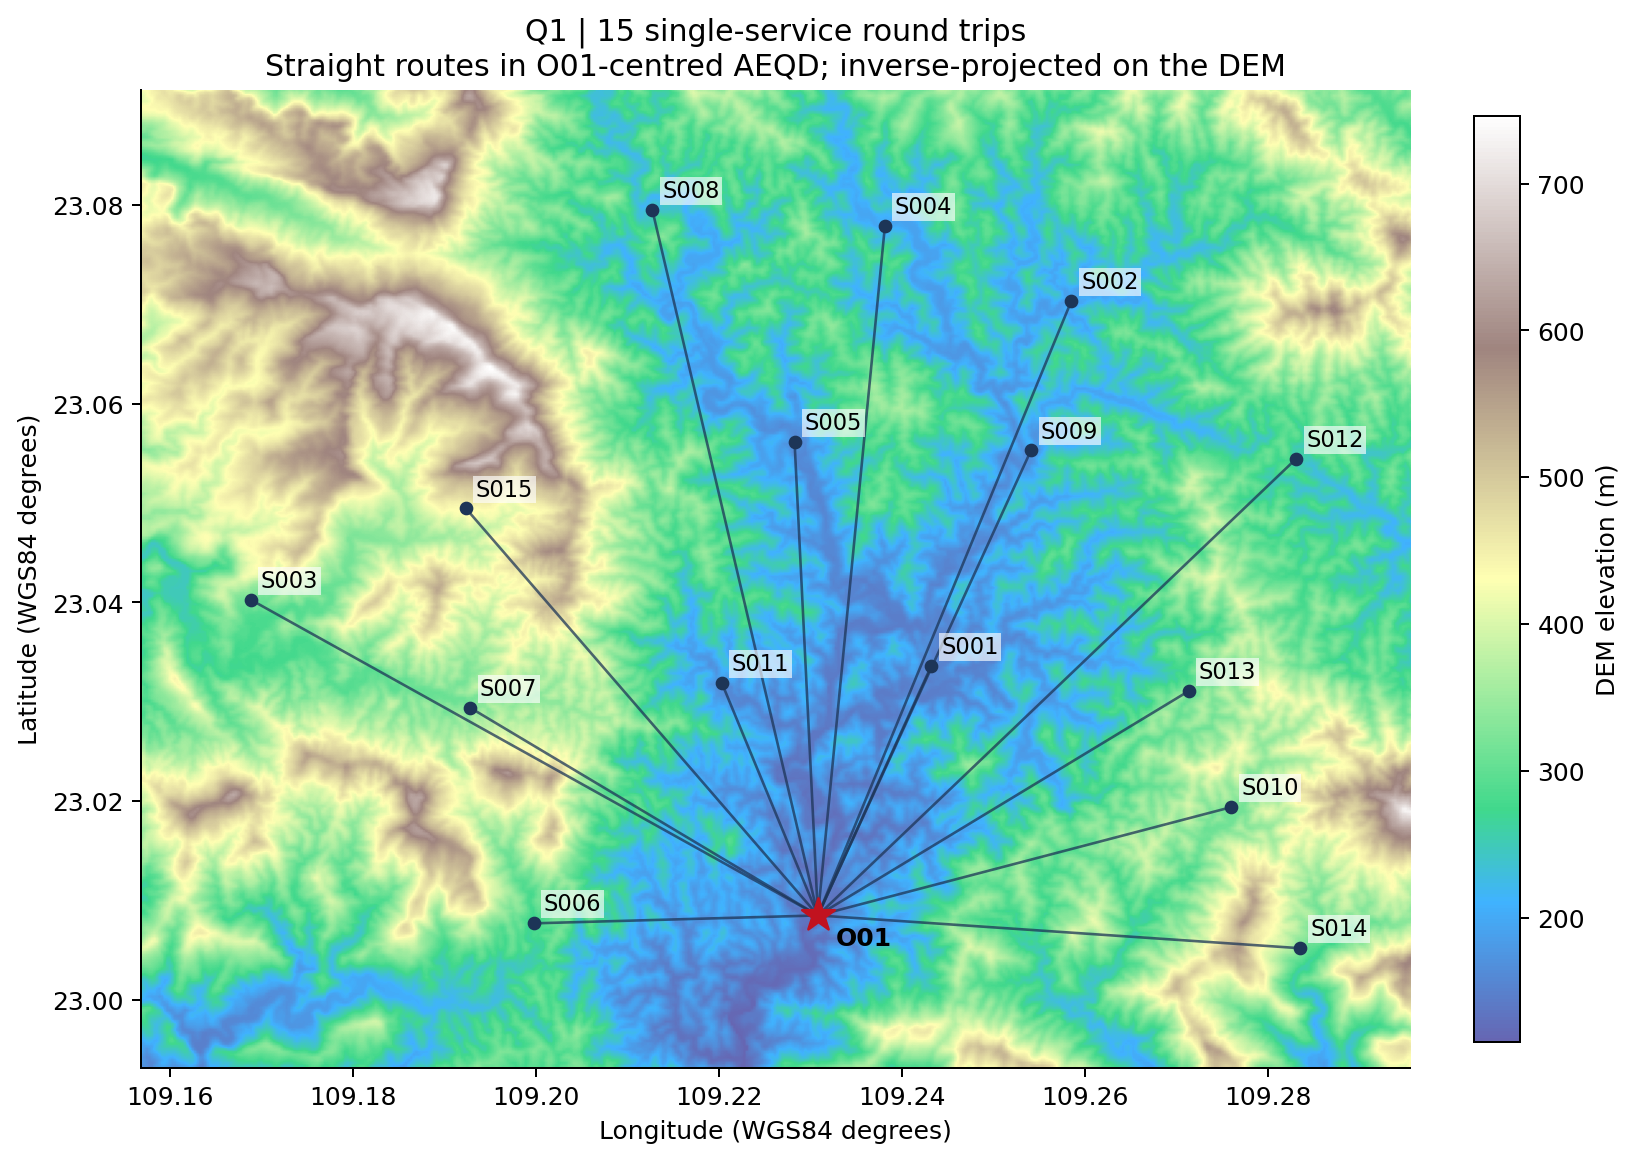
\includegraphics[width=0.82\textwidth]{map_single_routes.png}
  \caption{Q1基地O01至15个服务区的单点往返航线与DEM背景示意。该图仅用于空间关系展示，正式地形计算采用完整DEM像元相交。}
  \label{fig:app_q1_routes}
\end{figure}

\subsection{基线与Pareto结果}

\begin{table}[H]
\centering
\caption{Q1主要基线与正式方案}
\label{tab:app_q1_baseline}
\begin{tabular}{llrrr}
\toprule
机型策略 & 方法 & 架次 & 能耗/kWh & 累计作业时间/min\\
\midrule
A-only & exact & 52 & 112.180153 & 1488.763007\\
B-only & exact & 35 & 68.350657 & 927.625473\\
C-only & exact & 18 & 73.934908 & 563.979235\\
mixed & FFD-mass & 18 & 75.116697 & 563.979235\\
mixed & exact & 18 & \textbf{59.131296} & \textbf{546.266929}\\
\bottomrule
\end{tabular}
\end{table}

完整不同Pareto目标向量仅有两组：
\[
(18,\ 59.131296022053,\ 546.266929148593),
\]
\[
(19,\ 59.033942092203,\ 573.999623452513).
\]

\subsection{改变全局最少架次数的安全余量阈值}

\begin{table}[H]
\centering
\caption{Q1八个全局架次数临界阈值}
\label{tab:app_q1_thresholds}
\begin{tabular}{lcrr}
\toprule
安全余量阈值/\% & 触发区域 & 阈值处架次 & 严格右侧\\
\midrule
23.088350 & S004 & 18 & 19\\
27.049854 & S008 & 19 & 20\\
33.625809 & S008 & 20 & 21\\
33.896918 & S003 & 21 & 22\\
34.373532 & S004 & 22 & 23\\
34.391873 & S002 & 23 & 24\\
34.777897 & S008 & 24 & 25\\
35.267807 & S008 & 25 & 不可行\\
\bottomrule
\end{tabular}
\end{table}

完整569个候选事件与19次词典序最优代表变化由 \path{problems/D/q1/results/reserve_thresholds.csv} 和 \path{problems/D/q1/results/reserve_optimal_segments.csv} 保存。

% ============================================================
\section{问题二任务构造、调度结果与认证证据}
\label{app:q2}

\subsection{23个正式运输任务}

表\ref{tab:app_q2_tasks}直接对应 \path{q2_final/solution/main_23/decisions.json}。任务编号T01--T23仅用于论文展示，原始箱号保持不变。

\scriptsize
\begin{longtable}{cllp{8.2cm}}
\caption{Q2正式23个运输任务构成}\label{tab:app_q2_tasks}\\
\toprule
任务 & 机型 & 访问顺序 & 原始货箱ID\\
\midrule
\endfirsthead
\toprule
任务 & 机型 & 访问顺序 & 原始货箱ID\\
\midrule
\endhead
T01 & C & S001 & S001-MED-01, S001-MED-02, S001-WAT-06, S001-WAT-07, S001-WAT-08, S001-FOD-03, S001-HYG-01, S001-HYG-02\\
T02 & C & S001 & S001-WAT-02, S001-WAT-03, S001-WAT-04, S001-WAT-05, S001-FOD-02\\
T03 & B & S010 & S010-MED-01, S010-WAT-01, S010-FOD-01\\
T04 & B & S014 & S014-MED-01, S014-WAT-01, S014-FOD-01\\
T05 & B & S012 & S012-MED-01, S012-WAT-01, S012-FOD-01\\
T06 & A & S001 & S001-WAT-01, S001-FOD-01\\
T07 & A & S004 & S004-WAT-01, S004-FOD-01\\
T08 & A & S013 & S013-WAT-01, S013-FOD-01\\
T09 & A & S011$\rightarrow$S004 & S004-MED-01, S004-WAT-02, S011-MED-01\\
T10 & C & S006 & S006-MED-01, S006-WAT-01, S006-WAT-02, S006-WAT-03, S006-FOD-01, S006-HYG-01\\
T11 & C & S002 & S002-MED-01, S002-WAT-02, S002-WAT-03, S002-WAT-04, S002-FOD-01, S002-FOD-02, S002-HYG-01\\
T12 & C & S007$\rightarrow$S003 & S003-WAT-02, S003-WAT-03, S003-WAT-04, S003-FOD-01, S003-FOD-02, S003-HYG-01, S007-HYG-01\\
T13 & C & S005 & S005-MED-01, S005-WAT-01, S005-WAT-02, S005-WAT-03, S005-FOD-01, S005-HYG-01\\
T14 & A & S009$\rightarrow$S002$\rightarrow$S013 & S002-WAT-01, S009-MED-01, S013-MED-01\\
T15 & A & S007 & S007-MED-01, S007-WAT-01\\
T16 & A & S007 & S007-WAT-02, S007-FOD-01\\
T17 & B & S004 & S004-WAT-03, S004-HYG-01\\
T18 & B & S008 & S008-MED-01, S008-WAT-01, S008-FOD-01\\
T19 & B & S008 & S008-WAT-02, S008-HYG-01\\
T20 & A & S003$\rightarrow$S015 & S003-MED-01, S003-WAT-01, S015-MED-01\\
T21 & A & S015 & S015-WAT-01, S015-FOD-01\\
T22 & A & S009 & S009-WAT-01, S009-FOD-01\\
T23 & A & S011 & S011-WAT-01, S011-FOD-01\\
\bottomrule
\end{longtable}
\normalsize

\subsection{正式主方案与22架次见证}

\begin{table}[H]
\centering
\caption{Q2正式23架次方案与22架次可行见证}
\label{tab:app_q2_22_23}
\begin{tabular}{lrr}
\toprule
指标 & 正式23架次 & 22架次见证\\
\midrule
A/B/C架次 & 11/6/6 & 11/4/7\\
加权迟到/s & 0 & 0\\
makespan/s & 5693.231489 & 7767.058323\\
总能耗/kWh & 66.214460 & 66.323024\\
最紧硬截止余量/s & 202.096058 & 645.017134\\
最低返航SOC/\% & 20.097383 & 20.097383\\
\bottomrule
\end{tabular}
\end{table}

22架次方案只证明“22架次可行”，不证明22架次的最小makespan，也不能据此推出所有22架次方案均慢于23架次主方案。

\subsection{V7全局有效上下界}

\begin{table}[H]
\centering
\caption{Q2-EVIDENCE-V7-FOCUSED认证摘要}
\label{tab:app_q2_v7}
\begin{tabular}{lr}
\toprule
证据项 & 数值\\
\midrule
全局有效下界/s & 5433.956428\\
认证可行上界/s & 5693.231490\\
区间宽度/s & 259.275062\\
UB归一化间隙 & 4.554093092\%\\
互补分支数 & 809\\
叶证书数 & 810\\
完整机型定价调用 & 2430\\
审计失败数 & 0\\
原问题makespan全局最优 & 未证明\\
\bottomrule
\end{tabular}
\end{table}



\subsection{有限邻域与计算层负结果}

围绕当前主方案共检查330个定向局部邻域，329个有限模型返回不可行，1个达到时限后保持未知；不能将该结果解释为原问题局部或全局最优证明。pricing dominance实验只评价固定真实定价输入：24个输入的各组中位耗时之和由6.323099 s降至2.026581 s，比值为3.1201；生成标签由5,706,982降至2,061,175，最小约化成本保持一致。该3.1201倍不是整个Q2求解器速度比。

% ============================================================
\section{问题三运输--中继联合方案与验证}
\label{app:q3}

\subsection{当前正式release摘要}

当前正式版本为 \texttt{Q3-BOTTLENECK-V6/time}，物理模型版本为 \texttt{Q3-HOVER-COMPATIBLE-V5}。

\begin{table}[H]
\centering
\caption{Q3 V6正式主方案摘要}
\label{tab:app_q3_summary}
\begin{tabular}{lr}
\toprule
指标 & 数值\\
\midrule
运输架次 & 23\\
中继架次 & 4\\
实体运输无人机 & 8\\
运输电池 & 14\\
中继无人机 & 2\\
中继能源组件 & 3\\
联合最后返航/s & 5836.969929\\
运输能耗/kWh & 66.251280\\
中继能耗/kWh & 2.688136\\
总能耗/kWh & 68.939416\\
加权迟到 & 0\\
硬迟到箱数 & 0\\
最小硬截止余量/s & 360.866938\\
最低运输返航SOC/\% & 20.097383\\
\bottomrule
\end{tabular}
\end{table}

\subsection{中继转场高度口径}

中继转场采用
\[
H_R(p)=\max\left\{\max_{c\in\mathcal C(O01,p)}Z(c)+50,\ z_p,\ z_{O01}\right\}.
\]
该规则只作用于中继往返转场，普通运输航段仍使用沿线最高地形+50 m。旧release中将悬停高度额外截断在地形净空巡航面以下，因此其有限候选域证书不能自动继承到V6。

\subsection{连续通信验证}

V6主方案重新构造真实运输轨迹、完整中继需求区间与临界端点。主验证器完成17,756项物理、资源、区间和端点检查，失败0；独立时空点核验36,672点，未发现断链。保存证据包含700份完整区间证书和1,238份临界端点证书。

\subsection{关键保障切换}

关键C型运输任务在V5中从相对956.973974 s起必须依赖西侧中继；V6将此前段保障延长至1039.150288 s，同时使西侧中继提前5.821245 s就绪。两项共同解释约87.997559 s的同模型工期改善。该分析解释保存日程中的关键链，不构成原问题全局下界。

\subsection{时间--能耗与鲁棒备选}

\begin{table}[H]
\centering
\caption{Q3 V6已验证候选}
\label{tab:app_q3_robust}
\begin{tabular}{lrrr}
\toprule
方案 & 额外统一损耗/dB & 联合工期/s & 总能耗/kWh\\
\midrule
time & 0 & 5836.969929 & 68.939416\\
energy & 0 & 5911.548135 & 68.735791\\
robust025 & 0.25 & 5866.140527 & 69.031751\\
q4\_tradeoff & 0 & 5866.140527 & 68.975497\\
\bottomrule
\end{tabular}
\end{table}

旧+0.50/+0.55 dB结果属于历史release，不属于V6；当前只把+0.25 dB方案作为V6下完整核验的通信裕度备选。

% ============================================================
\section{问题四V6严格分区与资源向量}
\label{app:q4}

\subsection{严格模型不可拆块}

冻结Q3 V6/time任务、绝对时刻和实际通信保障关系后，严格模型形成
\[
B_1=\{S001\},\qquad
B_2=\{S002,S003,S004,S005,S007,S008,S009,S010,S011,S012,S013,S014,S015\},\qquad
B_3=\{S006\}.
\]
严格两组共有3种无标签分区，严格三组只有1种。

\subsection{当前正式资源向量}

\begin{table}[H]
\centering
\caption{Q4 V6严格分类型资源需求与库存}
\label{tab:app_q4_vectors}
\begin{tabular}{lrrrr}
\toprule
资源类型 & 原库存 & 全局共享 & 严格K2 & 严格K3\\
\midrule
A型运输机 & 4 & 4 & 4 & 5\\
B型运输机 & 2 & 2 & 2 & 2\\
C型运输机 & 2 & 2 & 3 & 5\\
A型电池 & 6 & 6 & 6 & 7\\
B型电池 & 4 & 4 & 4 & 4\\
C型电池 & 4 & 4 & 4 & 6\\
中继无人机 & 2 & 2 & 2 & 2\\
中继能源组件 & 6 & 3 & 3 & 3\\
\midrule
总配置 & 30 & 27 & 28 & 34\\
\bottomrule
\end{tabular}
\end{table}

严格两组的正式需求和缺口为
\[
\mathbf D^{(2)}=(4,2,3,6,4,4,2,3),\qquad
\boxed{\mathbf G^{(2)}=(0,0,1,0,0,0,0,0)}.
\]
严格三组的需求和缺口为
\[
\mathbf D^{(3)}=(5,2,5,7,4,6,2,3),\qquad
\boxed{\mathbf G^{(3)}=(1,0,3,1,0,2,0,0)}.
\]

两组正式分区为“除S006外14区 / S006”，总缺口1；三组唯一分区为“S001 / 其余13区 / S006”，总缺口7。

\subsection{跨问折中}

V6另保留一个 \texttt{q4\_tradeoff} 候选：联合工期5866.140527 s、总能耗68.975497 kWh，其严格三组缺口为6。它在Q3时间--能耗二维上不优于正式time方案，但说明Q3最短工期与Q4最少独立配置并不等价。

\subsection{历史敏感性边界}

旧Q4-SENSITIVITY-V2中的relay-copy、N-1、Pareto和库存敏感性使用旧Q3日程，未针对V6重新计算。它们仍保留在仓库历史目录，但不能与当前V6 strict资源向量混用。

\subsection{资源最小数量的交叉核验}

对固定任务组和固定资源类型，最小资源数量
\[
N_{gp}^{\min}=\max_t n_{gp}(t)
\]
由事件扫描和半开区间峰值计算得到，并在V6完整运行包中以实体资源链和独立最大匹配进行交叉核验。

% ============================================================

\section{复现、版本锁与证据清单}
\label{app:repro}

\subsection{正式版本入口}

\begin{table}[H]
\centering
\caption{四问正式结果入口}
\label{tab:app_release}
\begin{tabular}{lll}
\toprule
问题 & 正式版本/提交 & 论文复现入口\\
\midrule
Q1 & \texttt{f905acc8482966c...} & \path{problems/D/q1/}\\
Q2 & Q2-EVIDENCE-V7-FOCUSED & \path{problems/D/q2/evidence_v7/}\\
Q3 & Q3-BOTTLENECK-V6 / time & \path{problems/D/q3/release_v6/time/}\\
Q4 & Q4-STRICT-FROM-Q3-V6 & \path{problems/D/q4/results_q3_v6/}\\
\bottomrule
\end{tabular}
\end{table}

\subsection{哈希锁定的伴随归档}

\begin{longtable}{p{6.5cm}p{8.0cm}}
\caption{正式伴随归档SHA-256}\label{tab:app_archives}\\
\toprule
归档 & SHA-256\\
\midrule
\endfirsthead
\toprule
归档 & SHA-256\\
\midrule
\endhead
D题\_Q2定向证据强化V7\_源码证书与复核.zip &
\texttt{0804f989699dc506b3111dacc7408d9acdeb6e1115e7f32ec36934116de6ce58}\\
D题\_Q3正式封口\_FINAL\_源码结果与交接.zip &
\texttt{97f5ea8018a557d604bee87d6886675ecf7648f035e8df0f47f20ff6e7fbc56b}\\
D题\_Q4稳健性完善V2\_源码结果与验证.zip &
\texttt{9c8d1a6410c2de0a410318fc3525dc162613deabf4ba9dd1d59cdeb98437f5b4}\\
D题\_Q2外部方案复核\_代码明细与验证.zip &
\texttt{b41a0416313a123e734e01d7ca1672b99acee41f16edd79812302e1007610b77}\\
\bottomrule
\end{longtable}

\subsection{证据等级与最终提交前检查}

正式论文中只允许使用与证据强度相匹配的表述：
\begin{itemize}
  \item Q1最少18架次：原Q1模型下全局证明；
  \item Q2加权迟到0：第一层目标全局证明；
  \item Q2 makespan：有效全局下界与完整可行上界，未闭合；
  \item Q3 V6：连续区间/临界端点与独立重放证明保存方案完整可行；
  \item Q3固定结构：连续时间LP证明当前固定离散结构下的时序最优；
  \item Q3鲁棒性：仅$+0.25$ dB为当前V6完整可行见证，旧$+0.50/+0.55$ dB不继承；
  \item Q4 K2/K3：冻结Q3 V6/time日程后的strict完整分区枚举。
\end{itemize}

最终提交前应再次以 \path{paper_integration/FINAL_SELECTION.json} 为唯一选择入口，逐项核对正文、摘要、图表、附录和机器可读结果，避免旧版本数字残留。


\end{document}
